% -*-latex-*-
% Document name: usersguide.tex
% Creator: Rob MacLeod [macleod@cvrti.utah.edu]
% Creation Date: Wed Feb 21 23:50:38 2001
%%%%%%%%%%%%%%%%%%%%%%%%%%%%%%%%%%%%%%%%%%%%%%%%%%%%%%%%%%%%%%%%%%%%%%
\documentclass[11pt]{article}
\usepackage[]{fancyhdr}
\usepackage[]{usersguide}
\usepackage[]{graphics}
\usepackage[]{epsfig}
\usepackage[]{html}
\usepackage{makeidx}
\usepackage{citexp}
%\usepackage[]{makeindex}
\makeindex
%%%%%%%%%%%%%%%%%%%%%%%%%%%%%%%%%%%%%%%%%%%%%%%%%%%%%%%%%%%%%%%%%%%%%%
\begin{document}

% -*-latex-*-
% Markup for SCIRun Users guide.
%
\textheight 9.5in
\textwidth 7in
\topmargin -.50in
\oddsidemargin -.25in
\sloppy

% Fancy headings stuff
\pagestyle{fancy}
\headsep .08in
\footskip 25pt
\headheight 15pt
\setlength{\footrulewidth}{.8pt}
%\setlength{\headrulewidth}{.8pt}
\rhead{{ \PSE{} Users' Manual}}
\lhead{Version \version}
\lfoot{}
\cfoot{}
\rfoot{{\small \sf Page: \hspace{1em}\thepage\hspace{1em}}}

% Setting to control figure placement.
% These determine the rules used to place floating objects like figures 
% They are only guides, but read the manual to see the effect of each.
\renewcommand{\topfraction}{.8}
\renewcommand{\bottomfraction}{.8}
\renewcommand{\textfraction}{.1}

% Paragraph spacing
% This sets the spacing between paragraphs
\setlength{\parskip}{\smallskipamount} 

% Common markup commands
% -*-latex-*-
%
%  For more information, please see: http://software.sci.utah.edu
% 
%  The MIT License
% 
%  Copyright (c) 2004 Scientific Computing and Imaging Institute,
%  University of Utah.
% 
%  License for the specific language governing rights and limitations under
%  Permission is hereby granted, free of charge, to any person obtaining a
%  copy of this software and associated documentation files (the "Software"),
%  to deal in the Software without restriction, including without limitation
%  the rights to use, copy, modify, merge, publish, distribute, sublicense,
%  and/or sell copies of the Software, and to permit persons to whom the
%  Software is furnished to do so, subject to the following conditions:
% 
%  The above copyright notice and this permission notice shall be included
%  in all copies or substantial portions of the Software.
% 
%  THE SOFTWARE IS PROVIDED "AS IS", WITHOUT WARRANTY OF ANY KIND, EXPRESS
%  OR IMPLIED, INCLUDING BUT NOT LIMITED TO THE WARRANTIES OF MERCHANTABILITY,
%  FITNESS FOR A PARTICULAR PURPOSE AND NONINFRINGEMENT. IN NO EVENT SHALL
%  THE AUTHORS OR COPYRIGHT HOLDERS BE LIABLE FOR ANY CLAIM, DAMAGES OR OTHER
%  LIABILITY, WHETHER IN AN ACTION OF CONTRACT, TORT OR OTHERWISE, ARISING
%  FROM, OUT OF OR IN CONNECTION WITH THE SOFTWARE OR THE USE OR OTHER
%  DEALINGS IN THE SOFTWARE.
%


%
% Latex package to be used by scirun documents.  Markup commands exist
% in two files.  This one and scirun-doc.tex.  This file contains
% commands that are processed by both latex and by the builtin
% capabilities of latex2html.  Scirun-doc.sty contains commands that are
% either completely ignored by latex2html or are processed by functions in
% the latex2html extension file scirun-doc.perl.
%
% Documents should include the
% following latex commands:
%
% \usepackage{scirun-doc}
% % -*-latex-*-
%
%  For more information, please see: http://software.sci.utah.edu
% 
%  The MIT License
% 
%  Copyright (c) 2004 Scientific Computing and Imaging Institute,
%  University of Utah.
% 
%  License for the specific language governing rights and limitations under
%  Permission is hereby granted, free of charge, to any person obtaining a
%  copy of this software and associated documentation files (the "Software"),
%  to deal in the Software without restriction, including without limitation
%  the rights to use, copy, modify, merge, publish, distribute, sublicense,
%  and/or sell copies of the Software, and to permit persons to whom the
%  Software is furnished to do so, subject to the following conditions:
% 
%  The above copyright notice and this permission notice shall be included
%  in all copies or substantial portions of the Software.
% 
%  THE SOFTWARE IS PROVIDED "AS IS", WITHOUT WARRANTY OF ANY KIND, EXPRESS
%  OR IMPLIED, INCLUDING BUT NOT LIMITED TO THE WARRANTIES OF MERCHANTABILITY,
%  FITNESS FOR A PARTICULAR PURPOSE AND NONINFRINGEMENT. IN NO EVENT SHALL
%  THE AUTHORS OR COPYRIGHT HOLDERS BE LIABLE FOR ANY CLAIM, DAMAGES OR OTHER
%  LIABILITY, WHETHER IN AN ACTION OF CONTRACT, TORT OR OTHERWISE, ARISING
%  FROM, OUT OF OR IN CONNECTION WITH THE SOFTWARE OR THE USE OR OTHER
%  DEALINGS IN THE SOFTWARE.
%


%
% Latex package to be used by scirun documents.  Markup commands exist
% in two files.  This one and scirun-doc.tex.  This file contains
% commands that are processed by both latex and by the builtin
% capabilities of latex2html.  Scirun-doc.sty contains commands that are
% either completely ignored by latex2html or are processed by functions in
% the latex2html extension file scirun-doc.perl.
%
% Documents should include the
% following latex commands:
%
% \usepackage{scirun-doc}
% \input{scirun-doc.tex}
%

% (Mostly) Short cuts  ==============================
\newcommand{\SCI}{{\em SCI}}
\newcommand{\sci}{\SCI}
\newcommand{\scii}{SCI Institute}
\newcommand{\BIOPSE}{\textbf{BioPSE}}
\newcommand{\biopse}{\BIOPSE}
\newcommand{\SR}{\textbf{SCIRun}}
\newcommand{\sr}{\SR}
\newcommand{\eg}{{\em e.g.,}}
\newcommand{\ie}{{\em i.e.,}}
\newcommand{\etc}{{\em etc.}}
\newcommand{\etal}{{\em et al.}}
\newcommand{\degrees}{{$^{\circ}$}}
\newcommand{\splitline}{\begin{center}\rule{\columnwidth}{.7mm}\end{center}}
\newcommand{\X}[1]{#1\index{#1}}
\newcommand{\srig}{\sr{} Installation Guide}
\newcommand{\srug}{\sr{} User's Guide}
\newcommand{\srdg}{\sr{} Developer's Guide}

% Literal ~ character
\newcommand{\ltilde}{\textasciitilde}

% Encloses its argument between angle brackets.
\newcommand{\ab}[1]{\textless{}#1\textgreater}

% Inserts a left angle bracket.
\newcommand{\la}{\textless}

% Inserts a right angle bracket.
\newcommand{\ra}{\textgreater}


% Mark up commands =================================

% Url
%\newcommand{\url}[1]{#1}

% ip address
\newcommand{\ipaddr}[1]{#1}
\newcommand{\localhost}{\ipaddr{127.0.0.1}}

% Predefined acronyms
\newcommand{\gui}{\acronym{GUI}}
\newcommand{\tcl}{\acronym{TCL}}
\newcommand{\xml}{\acronym{XML}}
\newcommand{\pse}{\acronym{PSE}}

% Markup the first time use of term that may be unfamiliar to the
% reader. 
\newmucmd{dfn}{emph}

% In the next command #1 is the term and #2 is the shortcut or acronym that
% will be used in the rest of the document. 
\newcommand{\dfna}[2]{\emph{#1} (\acronym{#2})}

% Markup a file name.
\newmucmd{filename}{texttt}

% Directory name markup.
\newmucmd{directory}{texttt}

% Markup text which is the name of a command.
\newmucmd{command}{texttt} 

% Command option.
\newmucmd{option}{texttt}

% Markup text typed at the keyboard.
\newmucmd{keyboard}{texttt} 

% Parameterized text - marks up text that is to be
% substituted for by the reader.
\newmucmd{ptext}{textit}        % Obsolete-use replaceable instead.
\newmucmd{replaceable}{textit}

% Markup text the user might see on his screen.
\newmucmd{screen}{texttt}

% Markup the name of a GUI menu.
\newmucmd{guimenu}{textbf}

% Markup the name of a GUI menu.
\newcommand{\menu}[1]{\guimenu{#1}}

% Markup a gui menu item name.
\newmucmd{guimenuitem}{textbf}

% Markup a menu item name.
\newcommand{\menuitem}[1]{\guimenuitem{#1}}

% Markup name of a ui button.
\newmucmd{guibutton}{textbf}

% Markup name of a ui button.
\newcommand{\button}[1]{\guibutton{#1}}

% Markup name of a gui text item.
\newmucmd{guitext}{textit}

% Markup name of a gui label.
\newmucmd{guilabel}{textbf}

% GUI variable
\newmucmd{guivar}{texttt}

% Scirun port
\newmucmd{srport}{texttt}

% Sockets port
\newcommand{\port}[1]{\texttt{#1}}

% Socket
\newcommand{\socket}[2]{\texttt{#1:#2}}

% Variable
\newcommand{\variable}[1]{\texttt{#1}}

% Data type
\newcommand{\datatype}[1]{\texttt{#1}}

% Function
\newcommand{\function}[1]{\texttt{#1}}

% Markup an inline code fragment.
\newcommand{\icode}[1]{\texttt{#1}}

% Markup a module name.
\newcommand{\module}[1]{\texttt{#1}}

% Markup a sr package name.
\newcommand{\package}[1]{\texttt{#1}}

% Markup a sr category name.
\newcommand{\category}[1]{\texttt{#1}}

% Env variable markup.
\newmucmd{envvar}{texttt}

% Markup for the title of a book or article or whatever.
\newcommand{\etitle}[1]{\textit{#1}}

% Markup name of a latex section.  First arg is section name.  Second arg
% is section's label.  When processed with latex, the section
% name is emphasized.  When processed with latex2html section name is made
% into a link to section.
\newcommand{\secname}[2]{\latexhtml{\emph{#1}}{\htmlref{#1}{#2}}}

% Section ref command.  Use of this command
% in place of \ref to reference sections (subsections etc.) will
% create a more web friendly version of your document.
% The command's first argument is the link text (used only on the html
% page) and the second argument is the section's label
\newcommand{\secref}[2]{\hyperref[ref]{\emph{#1}}{Section~}{}{#2}}
\newcommand{\chref}[2]{\hyperref[ref]{\emph{#1}}{Chapter~}{}{#2}}

% An alternative sec ref command.  When processed by latex, this
% command generates text like this: #1 (Section~\ref{#2}).  When
% processed by latex2html, this command generates a normal link using
% #1 as the link text.
\newcommand{\secrefalt}[2]{\latexhtml{\etitle{#1} (Section~\ref{#2})}{\htmlref{#1}{#2}}}

% Create a link to a doc in the tree.  Create a relative link if processed by
% latex2html and a footnoted http url to the sci web site when processed by
% latex.   Note that the macro \treetop must be defined before using
% this macro.
\newcommand{\scidoclink}[2]{\htmladdnormallinkfoot{#1}{\latexhtml{\scisoftware/doc}{\treetop}/#2}}

% A latex command
\newcommand{\latexcommand}[1]{\texttt{\textbackslash#1}}

% A latex package
\newcommand{\latexpackage}[1]{\textit{#1}}

% Use these in place of missing content.
\newcommand{\missing}[1]{\emph{#1 - Coming Soon.}}

% Use this to make note of incomplete content.
\newcommand{\incomplete}{\emph{More Comming Soon.}}

% Mark up a mail address
\newmucmd{mailto}{texttt}

% Mark up an xml attribute
\newmucmd{xmlattrname}{texttt}
\newmucmd{xmlattrvalue}{texttt}

% Alternate item commands inside a description environment
\newcommand{\descitem}[1]{\item[#1]\latex{\mbox{}\\}}
\newcommand{\menudesc}[1]{\item[\menu{#1}]\latex{\mbox{}\\}}
\newcommand{\menuitemdesc}[1]{\item[\menuitem{#1}]\latex{\mbox{}\\}}
\newcommand{\buttondesc}[1]{\item[\button{#1}]\latex{\mbox{}\\}}

% Sci Urls ========================================= 

% www style urls.
\newcommand{\scisoftware}{http://software.sci.utah.edu}
\newcommand{\scisoftwareurl}{\scisoftware}
\newcommand{\sciurl}{http://www.sci.utah.edu}
\newcommand{\scidocurl}{\scisoftware{}/doc}
\newcommand{\scidocurlplus}[1]{\scisoftware{}/doc/#1}
\newcommand{\bugsurl}{\scisoftware{}/bugzilla}
\newcommand{\scisoftwarearchiveurl}{\scisoftware{}/archive\_entry.html}

%

% (Mostly) Short cuts  ==============================
\newcommand{\SCI}{{\em SCI}}
\newcommand{\sci}{\SCI}
\newcommand{\scii}{SCI Institute}
\newcommand{\BIOPSE}{\textbf{BioPSE}}
\newcommand{\biopse}{\BIOPSE}
\newcommand{\SR}{\textbf{SCIRun}}
\newcommand{\sr}{\SR}
\newcommand{\eg}{{\em e.g.,}}
\newcommand{\ie}{{\em i.e.,}}
\newcommand{\etc}{{\em etc.}}
\newcommand{\etal}{{\em et al.}}
\newcommand{\degrees}{{$^{\circ}$}}
\newcommand{\splitline}{\begin{center}\rule{\columnwidth}{.7mm}\end{center}}
\newcommand{\X}[1]{#1\index{#1}}
\newcommand{\srig}{\sr{} Installation Guide}
\newcommand{\srug}{\sr{} User's Guide}
\newcommand{\srdg}{\sr{} Developer's Guide}

% Literal ~ character
\newcommand{\ltilde}{\textasciitilde}

% Encloses its argument between angle brackets.
\newcommand{\ab}[1]{\textless{}#1\textgreater}

% Inserts a left angle bracket.
\newcommand{\la}{\textless}

% Inserts a right angle bracket.
\newcommand{\ra}{\textgreater}


% Mark up commands =================================

% Url
%\newcommand{\url}[1]{#1}

% ip address
\newcommand{\ipaddr}[1]{#1}
\newcommand{\localhost}{\ipaddr{127.0.0.1}}

% Predefined acronyms
\newcommand{\gui}{\acronym{GUI}}
\newcommand{\tcl}{\acronym{TCL}}
\newcommand{\xml}{\acronym{XML}}
\newcommand{\pse}{\acronym{PSE}}

% Markup the first time use of term that may be unfamiliar to the
% reader. 
\newmucmd{dfn}{emph}

% In the next command #1 is the term and #2 is the shortcut or acronym that
% will be used in the rest of the document. 
\newcommand{\dfna}[2]{\emph{#1} (\acronym{#2})}

% Markup a file name.
\newmucmd{filename}{texttt}

% Directory name markup.
\newmucmd{directory}{texttt}

% Markup text which is the name of a command.
\newmucmd{command}{texttt} 

% Command option.
\newmucmd{option}{texttt}

% Markup text typed at the keyboard.
\newmucmd{keyboard}{texttt} 

% Parameterized text - marks up text that is to be
% substituted for by the reader.
\newmucmd{ptext}{textit}        % Obsolete-use replaceable instead.
\newmucmd{replaceable}{textit}

% Markup text the user might see on his screen.
\newmucmd{screen}{texttt}

% Markup the name of a GUI menu.
\newmucmd{guimenu}{textbf}

% Markup the name of a GUI menu.
\newcommand{\menu}[1]{\guimenu{#1}}

% Markup a gui menu item name.
\newmucmd{guimenuitem}{textbf}

% Markup a menu item name.
\newcommand{\menuitem}[1]{\guimenuitem{#1}}

% Markup name of a ui button.
\newmucmd{guibutton}{textbf}

% Markup name of a ui button.
\newcommand{\button}[1]{\guibutton{#1}}

% Markup name of a gui text item.
\newmucmd{guitext}{textit}

% Markup name of a gui label.
\newmucmd{guilabel}{textbf}

% GUI variable
\newmucmd{guivar}{texttt}

% Scirun port
\newmucmd{srport}{texttt}

% Sockets port
\newcommand{\port}[1]{\texttt{#1}}

% Socket
\newcommand{\socket}[2]{\texttt{#1:#2}}

% Variable
\newcommand{\variable}[1]{\texttt{#1}}

% Data type
\newcommand{\datatype}[1]{\texttt{#1}}

% Function
\newcommand{\function}[1]{\texttt{#1}}

% Markup an inline code fragment.
\newcommand{\icode}[1]{\texttt{#1}}

% Markup a module name.
\newcommand{\module}[1]{\texttt{#1}}

% Markup a sr package name.
\newcommand{\package}[1]{\texttt{#1}}

% Markup a sr category name.
\newcommand{\category}[1]{\texttt{#1}}

% Env variable markup.
\newmucmd{envvar}{texttt}

% Markup for the title of a book or article or whatever.
\newcommand{\etitle}[1]{\textit{#1}}

% Markup name of a latex section.  First arg is section name.  Second arg
% is section's label.  When processed with latex, the section
% name is emphasized.  When processed with latex2html section name is made
% into a link to section.
\newcommand{\secname}[2]{\latexhtml{\emph{#1}}{\htmlref{#1}{#2}}}

% Section ref command.  Use of this command
% in place of \ref to reference sections (subsections etc.) will
% create a more web friendly version of your document.
% The command's first argument is the link text (used only on the html
% page) and the second argument is the section's label
\newcommand{\secref}[2]{\hyperref[ref]{\emph{#1}}{Section~}{}{#2}}
\newcommand{\chref}[2]{\hyperref[ref]{\emph{#1}}{Chapter~}{}{#2}}

% An alternative sec ref command.  When processed by latex, this
% command generates text like this: #1 (Section~\ref{#2}).  When
% processed by latex2html, this command generates a normal link using
% #1 as the link text.
\newcommand{\secrefalt}[2]{\latexhtml{\etitle{#1} (Section~\ref{#2})}{\htmlref{#1}{#2}}}

% Create a link to a doc in the tree.  Create a relative link if processed by
% latex2html and a footnoted http url to the sci web site when processed by
% latex.   Note that the macro \treetop must be defined before using
% this macro.
\newcommand{\scidoclink}[2]{\htmladdnormallinkfoot{#1}{\latexhtml{\scisoftware/doc}{\treetop}/#2}}

% A latex command
\newcommand{\latexcommand}[1]{\texttt{\textbackslash#1}}

% A latex package
\newcommand{\latexpackage}[1]{\textit{#1}}

% Use these in place of missing content.
\newcommand{\missing}[1]{\emph{#1 - Coming Soon.}}

% Use this to make note of incomplete content.
\newcommand{\incomplete}{\emph{More Comming Soon.}}

% Mark up a mail address
\newmucmd{mailto}{texttt}

% Mark up an xml attribute
\newmucmd{xmlattrname}{texttt}
\newmucmd{xmlattrvalue}{texttt}

% Alternate item commands inside a description environment
\newcommand{\descitem}[1]{\item[#1]\latex{\mbox{}\\}}
\newcommand{\menudesc}[1]{\item[\menu{#1}]\latex{\mbox{}\\}}
\newcommand{\menuitemdesc}[1]{\item[\menuitem{#1}]\latex{\mbox{}\\}}
\newcommand{\buttondesc}[1]{\item[\button{#1}]\latex{\mbox{}\\}}

% Sci Urls ========================================= 

% www style urls.
\newcommand{\scisoftware}{http://software.sci.utah.edu}
\newcommand{\scisoftwareurl}{\scisoftware}
\newcommand{\sciurl}{http://www.sci.utah.edu}
\newcommand{\scidocurl}{\scisoftware{}/doc}
\newcommand{\scidocurlplus}[1]{\scisoftware{}/doc/#1}
\newcommand{\bugsurl}{\scisoftware{}/bugzilla}
\newcommand{\scisoftwarearchiveurl}{\scisoftware{}/archive\_entry.html}


% Users Guide specific markup
\newcommand{\version}{1.1}
\newcommand{\viewer}{\emph{Viewer}}

% Markup used by latex module descriptions.
\newcommand{\ModuleRef}[3]{\subsection{#1} #1 is in Category #2 of Package #3}
\newcommand{\Package}[1]{#1}
\newcommand{\Category}[1]{#1}
\newcommand{\Module}[1]{#1}
\newcommand{\ModuleRefSummary}{\subsubsection*{Summary}}
\newcommand{\ModuleRefUse}{\subsubsection*{Use}}
\newcommand{\ModuleRefDetails}{\subsubsection*{Details}}
\newcommand{\ModuleRefNotes}{\subsubsection*{Notes}}
\newcommand{\ModuleRefCredits}{\subsubsection*{Credits}}
\newcommand{\ModuleRefSubSection}[1]{\paragraph*{#1}}
\newcommand{\ModuleRefSubSubSection}[1]{\subparagraph*{#1}}
\newcommand{\ModuleRefFigName}[1]{#1}
\begin{rawhtml}

<!-- *************************************************************** -->
<!-- *************** STANDARD SCI RESEARCH HEADER ****************** -->
<!-- *************************************************************** -->
<center><img
SRC="http://www.sci.utah.edu/research/images/research_header_sm.gif"
usemap="#head-links" height="46" width="600" border="0"></center>
<map name="head-links">
        <area shape="rect" coords="491,15,567,32"
href="http://www.sci.utah.edu/research/research.html">
        <area shape="rect" coords="31,9,95,36" href="http://www.sci.utah.edu">
</map>
<!-- *************************************************************** -->
<!-- *************************************************************** -->

\end{rawhtml}

% The title page
% -*-latex-*-
%
%  The contents of this file are subject to the University of Utah Public
%  License (the "License"); you may not use this file except in compliance
%  with the License.
%
%  Software distributed under the License is distributed on an "AS IS"
%  basis, WITHOUT WARRANTY OF ANY KIND, either express or implied. See the
%  License for the specific language governing rights and limitations under
%  the License.
%
%  The Original Source Code is SCIRun, released March 12, 2001.
%
%  The Original Source Code was developed by the University of Utah.
%  Portions created by UNIVERSITY are Copyright (C) 2001, 1994
%  University of Utah. All Rights Reserved.
%
%%%%%%%%%%%%%%%%%%%%%%%%%%%%%%%%%%%%%%%%%%%%%%%%%%%%%%%%%%%%%%%%%%%%%%
  \mbox{}
  \vspace{2in}
\begin{center}
   {\huge\bf \PSE{} User's Guide}\\
     \vspace{.5in}
     {\Large Version \version{} \\
     \medskip
     Last update: \today \\}
     \bigskip
     {\Large Authors: \htmladdnormallink{\rob{}}
     {mailto:macleod@cvrti.utah.edu}, \\
     \htmladdnormallink{\ted{}}
     {mailto:dustman@cvrti.utah.edu}, \\
     and the SCI Gang\\}
  \bigskip

     {\Large 
     Scientific and Computing Institute (SCI)\\
     \htmladdnormallink{www.sci.utah.edu}{http://www.sci.utah.edu/}\\
     \medskip
     Nora Eccles Harrison \\
     Cardiovascular Research and Training Institute (CVRTI)\\
  %   \smallskip
     \htmladdnormallink{www.cvrti.utah.edu}{http://www.cvrti.utah.edu/}\\
     \medskip

     \bigskip
     Support for this project came from:\\
     \medskip
     The NIH National Center for Research Resources  
     \htmladdnormallink{(NCRR)}{http://www.ncrr.nih.gov}}

\end{center}

%%% Local Variables: 
%%% mode: latex
%%% TeX-master: "usersguide"
%%% End: 

\newpage
\tableofcontents
\newpage

% Now the main sections of the manual
% -*-latex-*-
%
%  The contents of this file are subject to the University of Utah Public
%  License (the "License"); you may not use this file except in compliance
%  with the License.
%
%  Software distributed under the License is distributed on an "AS IS"
%  basis, WITHOUT WARRANTY OF ANY KIND, either express or implied. See the
%  License for the specific language governing rights and limitations under
%  the License.
%
%  The Original Source Code is SCIRun, released March 12, 2001.
%
%  The Original Source Code was developed by the University of Utah.
%  Portions created by UNIVERSITY are Copyright (C) 2001, 1994
%  University of Utah. All Rights Reserved.
%

% intro.tex
%

\section{Introduction}
\label{sec:intro}


This is the \etitle{\srug}.  It describes the purpose and use, of the \sr{}
problem solving environment.  It is for those users who will be building
and executing \dfn{networks} within the \sr{} environment.

Those who will be installing \sr{} should read the
\htmladdnormallinkfoot{\srig{}}{\installguideurl}.


%\subsection{Conventions}
%\label{sec:conventions}

%\missing{Discussion of typographic conventions}

\subsection{Road Map}
\label{sec:roadmap}

This document is organized into the following main sections:

\begin{description}
  \item \secref{Introduction}{sec:intro} is what you are reading now.
  \item \secref{Concepts}{sec:concepts} introduces the concept of an
        integrated problem solving environment  and describes how \SR{}
        embodies some of these ideas.
  \item \secref{Starting \sr}{sec:startingup}  outlines the procedure for
        starting \sr{} and related information.
  \item \secref{Working with Networks}{sec:workwithnets} discusses tasks
        involved in building, editing, and executing networks.
  \item \secref{Visualization with the \viewer{}}{sec:viewer} describes the
        purpose and use of a visualization module called the \viewer{}.  The
        \viewer{} is probably \sr{}'s most commonly used module.
  \item \secref{Packages}{sec:packages} offers an overview of the content
        of the \sr{} and \pse{} packages (which provide nearly all of
        \sr{}'s computational services).
  \item \secref{Importing data into \sr{}}{sec:import} summarize ways to
        get data in your local format into and out of \SR{}.
\end{description}

\subsection{Getting Help}
\label{sec:help}

Help is available from several sources.

\subsubsection{In the Distribution}

This document and others related to \sr{} can be found in your \sr{}
distribution.  Point your browser at \filename{index.html} which is in your
distribution's top level \directory{doc} directory (\ie{} \ab{top of
distribution}/doc/index.html).  Latex and postscript versions of some
documents are also in the distribution's \directory{doc} directory.

\subsubsection{On the Web}

This and other documents related to \sr{} can be found in the
\htmladdnormallinkfoot{document}{\scidocurl{}} section of the
\htmladdnormallinkfoot{\sci{}}{\sciurl{}} web site.

Be sure to visit the main \sci{} web site for lots of other
information related to \sr{} and the \scii{}.

\subsubsection{From the Mailing Lists}

The \sr{} users mail list is a forum for discussing \sr{} related issues.
To subscribe send mail to:

\mailto{Majordomo@sci.utah.edu}

with the following command in the body of your message:

\keyboard{subscribe scirun-users}

\subsection{Reporting Bugs}
\label{sec:bugs}

Please report bugs!  To report a bug visit \sr{}'s
\htmladdnormallinkfoot{bug database}{\bugsurl} web page.

Reporting bugs this way (rather than by way of the mailing list) ensures
that they will be fixed in timely manner.



%%% Local Variables: 
%%% mode: latex
%%% TeX-master: "usersguide"
%%% End: 

% -*-latex-*-
%
%  The contents of this file are subject to the University of Utah Public
%  License (the "License"); you may not use this file except in compliance
%  with the License.
%
%  Software distributed under the License is distributed on an "AS IS"
%  basis, WITHOUT WARRANTY OF ANY KIND, either express or implied. See the
%  License for the specific language governing rights and limitations under
%  the License.
%
%  The Original Source Code is SCIRun, released March 12, 2001.
%
%  The Original Source Code was developed by the University of Utah.
%  Portions created by UNIVERSITY are Copyright (C) 2001, 1994
%  University of Utah. All Rights Reserved.
%

%%%%%%%%%%  Figures used in this file %%%%%%%%%%%%%%%%%%%%%%%%%%%%%%%%
%begin{latexonly}
  \newcommand{\basicmodule}%
  {\centerline{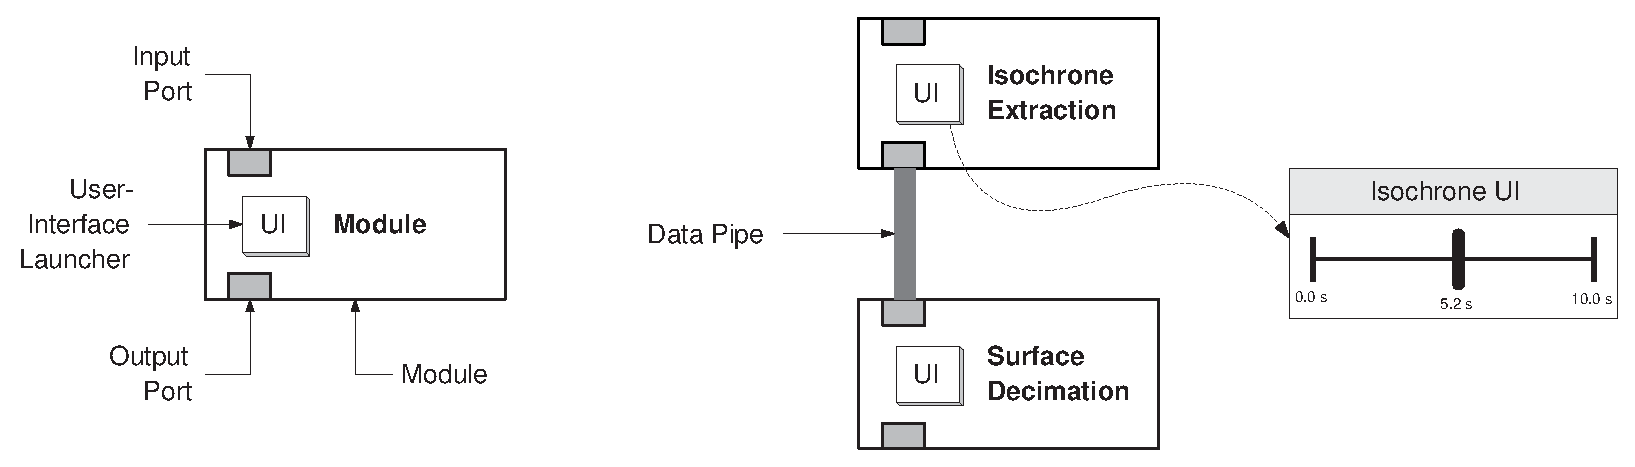
\epsfig{file=Figures/biopse-modmap.eps.gz,width=\columnwidth,
  bbllx=7, bblly=-193, bburx=774, bbury=14}}}
%end{latexonly}
\begin{htmlonly}
  \newcommand{\basicmodule}{%
  \htmladdimg[align=top,width=766,alt="module"]
  {../Figures/biopse-modmap.gif}}
\end{htmlonly}
%%%%%%%%%%%%%%%%%%%%%%%%%%%%%%%%%%%%%%%%%%%%%%%%%%%%%%%%%%%%%%%%%%%%%%
\section{Concepts}
\label{sec:concepts} 
\index{concepts}

Read this section to learn about the design philosphy and goals of
integrated problem solving environments \index{problem solving environment}
generally and how \PSE{} embodies
some of these ideas.  

\subsection{Traditional problem solving methods}

The traditional method for solving bioelectric field problems uses
multiple, non-integrated computer programs.  For example, a scientist using
a computer simulation to examine the effect of electrode patch placement on
transcardiac current density in the design of a cardiac implantable
defibrillator\cite{CRJ:Sch95b} would require geometric modeling, numerical
simulation, and scientific visualization tools to complete the task.  The
user might need one program to define the thoracic surfaces from medical
images and another to create a discrete mesh of the volume contained within
the surfaces\cite{CRJ:Sch93b}.  Another application like Matlab computes a
finite element simulation of the electric current distribution from the
defibrillation electrodes through the thoracic volume\cite{RSM:And93}.
Another approach might be to write a Fortran program using a public domain
numerical library such as LAPACK\@ \index{LAPACK}.  To see the output would
require a scientific visualization package (such as those described
in\cite{RSM:All91}).  Between each of these steps, it would be necessary to
save the output of one program in a format that the next in the sequence
could read---this might necessitate separate file format conversion
utilities.  To find the optimal location, shape, and size parameters for
the defibrillating electrode, the scientist would have to go back to the
geometric modeling package, change the necessary parameters, manually
re-run all of the subsequent steps to see how the new electrode
configuration affects the current density distribution, and then manually
iterate.  The manual intervention required to drive this process is both
tedious and time consuming.

Far more efficient is a scenario in which the user could define an
appropriate set of parameters for a given simulation, and then set up
a sequence of runs to examine each of them and save the results for
subsequent examinations.  The complete execution of the sequence might
require hours or even days, but the user would be free during that
time to perform other tasks.  This process is similar to the ``what
if?'' analysis that modern spreadsheet programs offer for much simpler
problems.  

In our example of the defibrillation simulation, the scientist could select
various locations and orientations for the defibrillation electrodes,
choose values for the other parameters of the simulation (\eg{} the number
of nodes in the finite element model, the boundary conditions, the error
tolerance for convergence, and the evaluation criteria), and leave the
simulations to run as long as necessary.  Viewing the results might be as
simple as watching the animation produced by the simulation or scanning
other defibrillation quality indices such as maximum and minimum current
density magnitude or current density histograms from the heart.  This
automated execution process, whereby the user selects all of the parameters
in advance and does not control the intra- or inter-package execution is
\emph{batch processing}.  A primary benefit of batch processing it that it
allows the scientist to utilize computational resources without the need to
continuously guide the process.  However, with most available computer
programs execution cannot be automated.  That is, the package cannot be run
without regular user intervention during execution.  This constraint makes
it difficult or impossible to run multiple computational jobs
automatically, leaving the user with the task of manually initiating and
controlling each step of the process.

\subsection{Integrated problem solving and computational
steering} 
\label{sec:con-steering} 

The goal of integrated problem solving environments---and specifically of
\SR{} and \PSE{}---is to incorporate and integrate all the steps described
in the previous example as components in a single, unified, extensible
problem solving environment (PSE)\index{PSE}.  The functionality that will
result includes the ability to manage each step in a sequential computing
process, and to create batch processes that execute repeated simulations.
However, the functionality that sets \SR{} and \PSE{} apart from most
integrated software environments is the ability to intervene and control
execution anywhere in the chain at any time during its execution.  This
ability to control a computer program during execution is termed
\emph{computational steering.}

To provide a non-technical analogy, adding computational steering to a
software environment is similar to adding the ability to occasionally
switch tracks to train travel.  A train passenger can get on the train and
automatically get to a new destination, leaving all the details of the
individual actions to the rail system machinery and staff.  But the route
and the destination are fixed.  Steering would permit each passenger to
request that the train take a new route, with different stops, and even a
different destination, and be able to make these decisions at any time
during the trip.  In the more rigorous example of the defibrillation
simulation, computational steering allows a scientist to interactively
change parameters and settings as the simulation executes, both as a single
run or in batch mode.  Steering interventions might include adjusting
electrode locations to stay within anatomically reasonable bounds or
refining the geometric model resolution in order to balance accuracy and
execution time.

To achieve integration within the elements of \SR{} and \PSE{}, data 
flows directly from one processing step to the next, without ever being
diverted to a disk file or leaving the program.  Output from any step 
are available as inputs to dependent steps.  The underlying paradigm of
\SR{} is of data flowing between modules that each perform some
operation.  Integration between modules guarantees that upon completion of
their tasks, upstream modules pass their data to downstream modules,
thereby forcing the downstream modules to execute in response.  In our
example, this means that the scientist may alter electrode locations at any
time, thus initiating a sequence of all the necessary steps to recompute
the simulation with the new configuration.  The modification of the
geometric model, finite element calculation, and visualization all proceed
automatically and in the proper sequence, all managed by \SR{}.  This
combination of steering and component integration allows the scientist
to spontaneously explore a problem.  

While computational steering is still a young field in computer science,
there are a number of examples of such systems (besides \SR{}) described in
the literature.  Burnett\cite{MM:Bur94}, and Vetter and
Schwan\cite{MM:Vet96} give overviews of existing computational steering
system.  Several notable examples include CUMULVS\cite{MM:Gei96,MM:Koh97},
\index{CUMULVS} Progress\cite{MM:Vet95}, \index{Progress} and
Magellan\cite{MM:Vet97a} \index{Magellan}.



\subsubsection{\SR{} versus \PSE{}}
\label{sec:srversuspse} 

It is important to understand the place of the software included in this
package within the hierarchy of computational problem solving environments
developed at the SCI Institute.  From a historical perspective, \SR{},
which we started developing in 1992, was the original implementation of the
computational
framework\cite{CRJ:Joh94c,RSM:Par95,RSM:Par95b,RSM:Par97,RSM:Par97b,CRJ:Parker99b}.
Since then, \SR{} and its computational workbench infrastructure have been
the origin of many significant application-specific projects.  Two major
examples are the DOE sponsored Uintah system \cite{RSM:Dav2000} and the NIH
sponsored \PSE{} system.  The target applications of the Uintah project are
combustion, computational fluid dynamics, and mechanical modeling
implemented on large-scale, distributed, shared memory architectures.  The
goal of the \PSE{} project is to create software for geometric modeling,
simulation, and visualization for solving bioelectric field problems.  An
important secondary goal of the \SR{} system is to make source code for
these problem solving environments publicly available to the scientific
community.

To realize these two significant projects, the \SR{} infrastructure itself
has required significant reorganization, extension, and enhancement.  Even
with these recent changes, \SR{} remains both the core infrastructure for
our problem solving environments and the name we use to refer to the entire
ensemble of software.  Thus a user may install and operate the core \SR{}
software and also augment its functionality with one or more of the
"packages" such as \PSE{}.  We anticipate that the collection of packages
will grow as the advantages of the \SR{} infrastructure become available
to scientists and engineers of all disciplines.

In addition to the major projects that have both leveraged and advanced
\SR{}, there exist a number of smaller packages that can extend \SR{}'s
utility.  Examples include the Teem package for raster data processing, the
NetSolve package for linear algebra subroutines (developed by researchers
at the University of Tennessee and Knoxville), and a communications
interface we have recently introduced to the Matlab program.  We have
developed various forms of software wrappers or interfaces that allow
\SR{} to leverage the strengths of these third party tools, links we refer
to as "bridges."

There are also instances in which a tighter level of integration than a
bridge between \SR{} and third-party software is necessary.  One example
is the addition of mpeg support for capturing animations from the \SR{}
Viewer module, for which we use the Berkeley and Alex Knowles' mpeg
encoding tools.  Another example is the set of image generation and
manipulation tools from Peter Haeberli called libimage.  To indicate
whether or not such tools are available, the configure scripts for \SR{}
contain optional control flags.

We believe that this combination of a robust infrastructure and modular
extensibility through packages and third-party libraries will allow \SR{}
to grow and adapt to changing needs and opportunities. 

In this manual, we will try and be consistent about the usage of the two
terms, \SR{} and \PSE{}.  \SR{} will typically refer to some feature that
is common to the core functionality of the system and this is common to all
of the problem solving environment applications packages.  \PSE{} will
refer to specific elements of the bioelectric field problem solving
environment.


\subsection{\SR{} modules and networks}
\label{sec:con-modules} 


\begin{figure}[htb]
  \begin{makeimage}
  \end{makeimage}
  \basicmodule
%  \centerline{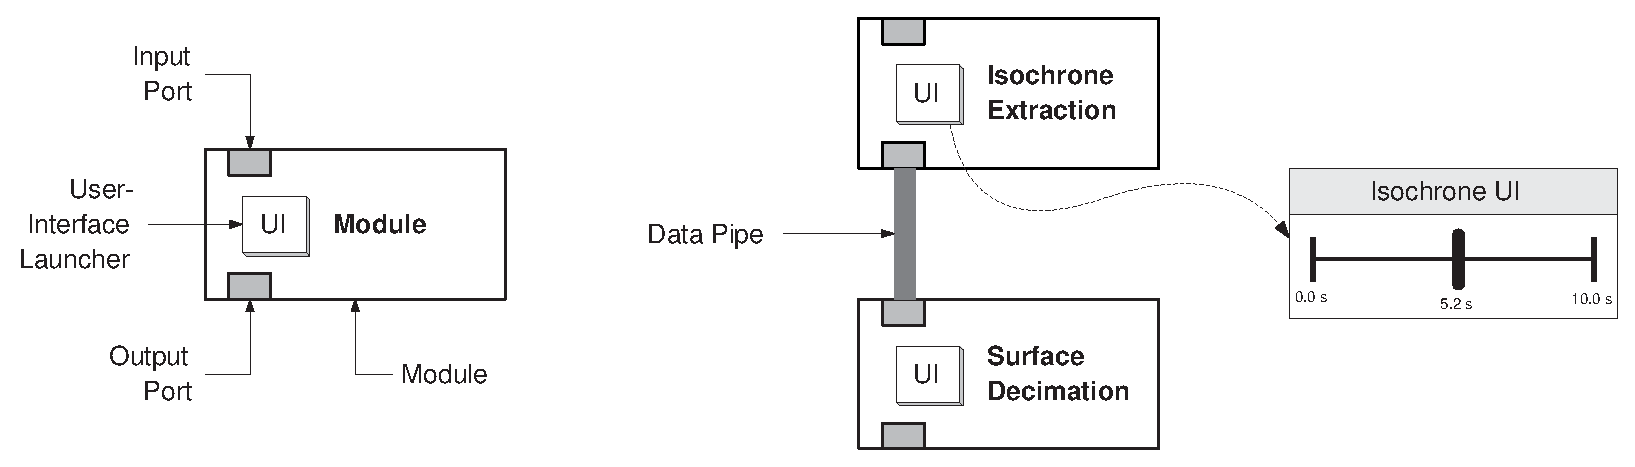
\epsfig{file=Figures/biopse-modmap.eps,width=6in}}
  \caption{\label{fig:conc-module} Example of a \SR{} module}
\end{figure}

The functional unit of a dataflow environment is the {\em\/module}
\index{module}.  Figure~\ref{fig:conc-module} contains a generic \SR{}
module, with a User Interface (UI) button for graphically accessing the
module's parameters, and input and output ports for receiving and sending
data, respectively.  On the right is a simple example of a dataflow
network.  Data passes through the output port of the top module, through
the data pipe, and into the input port of the bottom module.  The User
Interface enables the selection of a desired isochrone surface.

Modules may contain other elements, but they will all have at least one
input or one output port.  Examples of a module with only an output port
would be file readers.  The \htmladdnormallink{\emph{Viewer}}{viewer.html}
module contains only input ports because it receives information and the
output is a visualization.  For a more detailed description of modules and
how to control them, see \secref{Working with Networks}{sec:workwithnets}.
The most important goal at this stage is to appreciate the concept of a
module and the dataflow that links one module to another.

A network diagram \index{network!diagram} describes the way data flows
through \SR{} and is the main means of user interaction with the overall
action of the program.  The network essentially defines the basic function of
the program; without a network, \SR{} and \PSE{} are just a set of tools
sitting in a chest.  By joining the modules into a network, the tools
become a functioning program that does whatever the network tells it to.
Once again, the important thing to appreciate is what the network is
conceptually; for the details, see \secref{Working with
Networks}{sec:workwithnets}. 


\subsection{Links to third party software}
\label{sec:con-links} 

\SR{} works together with software from third party sources in several
ways.  If you have installed \SR{} and \PSE{} yourself, you will have seen
the need for some third party software libraries that are required for
basic functionality.  This type of third party software is largely
invisible to the user of \SR{} or \PSE{}, at least until something
breaks\ldots{} Perhaps the most evident is the
\htmladdnormallink{TCL/Tk}{http://www.tcltk.com/} \index{Tcl/Tk} library,
which \SR{} uses to create the network editor and the icons for the modules
and data pipes.  In fact, \SR{} is actually a large TCL script that calls a
lot of specialized C++ code to do all the hard work.


Far more interesting is the interaction between programs you may have that
are written in FORTRAN \index{FORTRAN} or
\htmladdnormallink{Matlab}{http://www.mathworks.com/products/matlab/} and
\SR{}.  One of the goals of the \PSE{} project was to develop support for
such external code, including FORTRAN, C, Matlab, and IDL\@.  This first
version of \PSE{} has support for Matlab and one example of wrapping
existing FORTRAN code into a \SR{} module. \index{Matlab}

\subsubsection{\SR{}/Matlab interface}
\label{sec:concept-matlab} 

The interface (based on Berkeley sockets) between \SR{} and Matlab provides
a pathway to send matrix data objects from \SR{} to Matlab and then accept
the result of some Matlab computations.  At present, this arrangement
requires that a Matlab script exist that will perform the desired
operations.  \SR{} sends the input data to an existing process running
Matlab, which serves as a compute engine, performs the steps
described in the script, and then returns data to \SR{} for further
processing or display.  The Matlab process can even run on a separate
computer connected via a network, which helps to distribute the load as
well as to resolve potential licensing conflicts with Matlab.

The underlying mechanism for this communication is a socket interface
consisting of two \SR{} Modules, \module{MatrixSend} and
\module{MatrixReceive}, and a Matlab ``transport'' routine.  Both the \SR{}
and the Matlab process know about each other's whereabouts (in the form
hostname:port) and use a client-to-client communication model, so that
synchronization between processes is manual.  For example, 
the \SR{} \module{MatrixSend} module sends the matrix to a socket at which a 
Matlab script is listening.  The script then receives the matrix, 
performs the calculations in Matlab and sends the results to a socket 
where \module{MatrixReceive} module is listening.  \SR then carries out
further calculations and display of the results.

%For examples of this interface, see \secref{Matlab
%Examples}{sec:examples-matlab}.

\subsubsection{Links to GENESIS}

\htmladdnormallink{GENESIS}{http://www.bbb.caltech.edu/GENESIS/genesis.html}
(short for GEneral NEural SImulation System) is a general purpose
simulation platform which was developed to support the simulation of neural
systems ranging from complex models of single neurons to simulations of
large networks made up of more abstract neuronal components. GENESIS has
provided the basis for laboratory courses in neural simulation at both
Caltech and the Marine Biological Laboratory in Woods Hole, MA, as well as
many other institutions.   

We have created a bridge between \SR{} and GENESIS so that it is possible
to use the output of a GENESIS simulation as the input for either a
visualization or a subsequent simulation within \PSE{}.  The mechanism for
this bridge is a database that is accessible via SQL queries.  We created
code for GENESIS that writes the output of the simulation into the database
and then the corresponding functions for \SR{} that will read this
information from the same database.  The details of this mechanism are a
work in progress so for details, please contact Chris Butson
\htmladdnormallink{Christopher.Butson@m.cc.utah.edu}
{mailto:Christopher.Butson@m.cc.utah.edu}.

\subsection{Extensibility}
\label{sec:con-extend} 

\SR{} is an extensible \index{extensible} problem solving environment.
This is true in the sense that no one by the user really limits the
different ways of connecting modules and creating new applications.  It is
also more generally true that \SR{} is designed to have users who can
program  their own new modules.  To support creating new modules, we
have developed the \emph{Module maker} application, described in 
\htmladdnormallink{The Module Maker manual}{\modulemakerguideurl}.

With the release of \SR{}, we anticipate that users all over the world will
create new modules and we will encourage them to contribute modules to a
repository on the \PSE{} web site \index{BioPSE@\PSE{}!web site}
(\htmladdnormallink{www.sci.utah.edu/ncrr/software/biopse.html}
{http://www.sci.utah.edu/ncrr/software/biopse.html}.  We will review
submissions to this collection of modules and adopt and then test generally
useful ones to include in subsequent releases of \PSE{}.  Future releases
will also include more extensive tools for both building modules and
wrapping existing codes within \SR{} module wrappers to maximize your
intellectual investment in legacy code.


\subsection{Detachable interface}
\label{sec:con-detach} 
\index{detachable interface}

A strategy seen in a few PSEs currently under development and an integral
part of \SR{} is the idea of a detachable interface.  Rather than having a
fixed link between a user interface and the underlying application, a
detachable interface can be separated from the application, in which case
the application becomes unsteerable.  The advantage, however, lies in the
ability to now re-attach an interface to a running application and thus
re-enable steering.  The re-attached interface need not be from the same
physical computer from which the application was started, instead it may
come from a remote computer via a network, or from another user on the same
computer.  An additional strength of this approach is that the re-attached
interface may not be an interactive widget at all, but a set of commands
executed from a script.  This permits complete remote control of the
application and thus is a flexible blend of interactive and almost
unlimited batch control.  CUMULVS \index{CUMULVS} is one example of such a
system and uses its detachable interface to allow collaboration between
scientists working remotely, with viewing systems that can attach or detach
from the running simulation.

The first release of \SR{} will not include any of the detachable interface
support but we plan to add this within six months of the first release.


%%% Local Variables: 
%%% mode: latex
%%% TeX-master: "usersguide"
%%% End: 

\newpage
% running.tex
%
% This is the `Running SCIRun' main section.

%begin{latexonly}
  \newcommand{\srwindow}%
  {\centerline{\epsfig{file=figures/srwindow-1.eps.gz, width=6in,
        bbllx=0, bblly=0, bburx=579, bbury=578}}}
%end{latexonly}
\begin{htmlonly}
  \newcommand{\srwindow}{%
  \htmladdimg[align=top,alt="SCIRun Window"]
  {../figures/srwindow-1.jpg}}
\end{htmlonly}


\section{Starting \sr{}}
\label{sec:startingup}

\subsection{The \command{scirun} Command}
\label{sec:sciruncmd}

Start \sr{} by typing \keyboard{scirun} in a terminal (\eg \command{xterm})
window.  \note{Don't start \sr{} in the background, \ie don't type
\keyboard{scirun \&}}.

The \command{scirun} command is located in the
\directory{src} directory of the \directory{\sr} install directory.  The
person who installed \sr{} can locate this command for you.


\begin{figure}[htb]
  \begin{makeimage}
  \end{makeimage}
  \srwindow
  \caption{\label{fig:srwindow} \sr{} Main Window}
\end{figure}


Typing \keyboard{scirun} with no arguments starts up \sr{} with a blank \sr{}
window as shown in Figure~\ref{fig:srwindow}.  The main features of this
window are discussed in \secref{Anatomy of the Main
  Window}{sec:windowanatomy}.

The \command{scirun} command may take 1 argument
which is the name of a \sr{} \dfn{network} \index{network} file (these
files have a \filename{.net} extension).  These files hold previously
defined \sr{} networks.  \sr{} will load the specified network.  Network
files will be discussed in a later section.

\sr{} may encounter errors during start up.  These will be displayed in
\sr{}'s error message pane (see Figure~\ref{fig:srwindow}).  These errors
should be \htmladdnormallink{reported}{\bugsurl} to the \sr{} development
team.  \latexonly{See \secref{Reporting Bugs}{sec:bugs} for information on
  reporting bugs.}

\subsection{Anatomy of the Main Window}
\label{sec:windowanatomy}

The \sr{} main window consists of 4 main components (see
Figure~\ref{fig:srwindow}): 

\begin{description}
\item[Menu Bar] The menu bar is used to load networks, save networks, quit
  \sr, create network modules, and perform other tasks.  The menu bar
  consists of the following menu items:

  \begin{description}
  \item[\menu{File}] The \menu{File} menu contains the following items:
    \begin{description}
    \item[Save] Saves the current network to a file.
    \item[Load] Loads a network from a file.
    \item[New] This sub-menu contains items of interest to developers only.
    \item[Add Info] Use this item to add network specific notes to
      the current network.  Notes should be used to document the purpose of
      the network.
    \item[Quit] Quits \sr.
    \end{description}
  \end{description}
  
  \begin{description}
  \item[\menu{SCIRun}] The \menu{SCIRun} menu is used to create modules
    (from the \sr{} package) for use in the network pane.  This menu is
    composed of sub-menus. Each sub-menu corresponds to a \dfn{category}
    \index{category} within the \sr{} package.  A category is a group of
    related modules.  Each menu item in a category sub-menu creates a
    specific module and places it in the network pane.  The network pane's
    pop-up menu (activated by clicking the right most mouse button when the
    mouse pointer is in the network pane) also provides access to the
    \menu{\sr{}} and \menu{\pse{}} (and possibly other) package menus.  An
    overview of the contents of the \sr{} package is given in \secref{The
      \pse{} Package}{sec:biopsepackage}.
  \end{description}

  \begin{description}
  \item[\menu{BioPSE}] The \menu{BioPSE} menu is used to create modules
    (from the \pse package) for use in the network pane.  It consists
    of category sub-menus and module menu items.   An overview of the
    contents of the \sr{} package is given in \secref{The SCIRun
      Package}{sec:srpackage}.
  \end{description}

  \begin{description}
  \item [\textit{Other Package Menus}] There may be other package
    menus if other packages have been installed.  They too will consist
    of category sub-menus and module menu items.
  \end{description}
  
\item[Navigator Pane] The Navigator Pane is located in the upper left
  corner of the main window (see Figure~\ref{fig:srwindow}). It is used to
  navigate complex networks.  The use of the Navigator Pane will be
  described in \secref{Navigating a Network}{sec:navnetwork}.
  
\item[Error Pane] Errors during program startup are displayed in the Error
  Pane.  It is located in the upper right corner of the main window(see
  Figure~\ref{fig:srwindow}).  Errors on startup may mean that \sr{} has
  been installed incorrectly or has been installed from a buggy
  distribution.  Please \hyperref{report}{(see Section~}{)}{sec:bugs} these
  errors.
  
\item[Network Pane] The Network Pane occupies the bottom of the main
  window(see Figure~\ref{fig:srwindow}).  It is used to build and execute
  networks.  \secref{Building Networks}{sec:workwithnets} discusses the use
  of this pane.

\end{description}

\subsection{The Terminal Window}
\label{sec:termwinapp}

After starting, \sr{} will also run a shell-like application in the
terminal window called the \dfn{\sr{} shell}.  The \sr{} shell displays the
prompt \screen{scirun\ra}.  This program is actually a modified \dfna{Tool
  Command Language}{TCL} shell program and it is possible to type in
\acronym{TCL}'ish \sr{} commands at the prompt. The use of this program
will be described in \hyperref{a later section}{Section~}{}{sec:termapp}.


\subsection{Environment Variables}
\label{sec:environ} 
\index{Environment Variables}

There are several environment variables that \sr{} uses to make it easier
to use.  These are all optional, but paying attention to them can make it
easier to find files during a \sr{} session and to improve performance via
remote connections.

\begin{description}
  \item{\envvar{SCIRUN\_DATA}}\mbox{}: ]
        \index{SCIRUN\_DATA}
        \label{sec:scirundata}
        The environment variable \envvar{SCIRUN\_DATA} specifies the
        default directory of \sr{} data files.  \sr will first look in this
        directory to find data and network files.  It affects the behavior
        of file browsing dialogs -- they will prompt for a file within the
        \envvar{SCIRUN\_DATA} directory (of course you may have the dialog
        look elsewhere).  This can be very handy when using shared
        datasets, like the one shipped with the software.  Many of the
        demonstration nets with the software also assume that
        \envvar{SCIRUN\_DATA} points to the location of these datasets.

  \item[\envvar{SCIRUN\_DATASET}}\mbox{}: ]\mbox{}
        \label{sec:scirundataset} 
        This variable refines the search for data files within the director
        pointed at by \envvar{SCIRUN\_DATA}.  By setting these two
        variables, one can easily select different data sets for the same
        network.  See the network files distributed with the software, for
        example \filename{forward-fem.net}, so examples of how to use these
        variables.  Some of the demonstration nets do require setting
        \envvar{SCIRUN\_DATASET} so see the documentation on those.

  \item[\envvar{DISPLAY}: ]\mbox{}
        As with other programs that require a second window, \sr{} uses the
        \envvar{DISPLAY} environment variable to determine where output
        goes.  While you may have your \envvar{DISPLAY} variable set
        automatically when using ssh (secure shell) to log into another
        computers, the encryption on this communication pathway makes for
        very slow response from \sr{}.  To greatly accelerate display, set
        the \envvar{DISPLAY} variable to your local computer.  Note that at
        this point, communication between the host computer and your own
        will not be encrypted and thus is insecure; unless you are entering
        a password, however, this is not usually a problem.  Also not that
        for this to work, your local computer has to be willing to host the
        \sr{} window; this may require the use of the \command{xhost}
        command so see appropriate documentation for X11 or speak to your
        local system administrator.
\end{description}



\subsection{Quitting or Exiting \sr{}}
\label{sec:stopping}

Quit \sr{} by selecting the \menuitem{Quit} item from the \menu{File} menu

\warning{Don't press \keyboard{control-c} to exit \sr.  Doing this will
drop you into a debugger which is probably not what you want to do}.


%%% Local Variables: 
%%% mode: latex
%%% TeX-master: "usersguide"
%%% End: 

% -*-latex-*-
%
%  The contents of this file are subject to the University of Utah Public
%  License (the "License"); you may not use this file except in compliance
%  with the License.
%
%  Software distributed under the License is distributed on an "AS IS"
%  basis, WITHOUT WARRANTY OF ANY KIND, either express or implied. See the
%  License for the specific language governing rights and limitations under
%  the License.
%
%  The Original Source Code is SCIRun, released March 12, 2001.
%
%  The Original Source Code was developed by the University of Utah.
%  Portions created by UNIVERSITY are Copyright (C) 2001, 1994
%  University of Utah. All Rights Reserved.
%

% network.tex
%

\section{Working with Networks}
\label{sec:workwithnets}

This section describes how to create, save, load, execute, and edit
networks.

When started with no arguments the \command{scirun} command will create a
main window with a blank NetEdit frame. The user creates and
connects modules to form a network.


\subsection{Creating a Module}
\label{sec:creatingmodules}

To create a module, select its name from one of the package (\eg{} \sr)
menus' category sub-menus.  The package menus may be accessed from the
main window's menu bar and from the NetEdit frame's pop-up menu. 
Activate the NetEdit frame's pop-up menu by clicking mouse button
3 while the mouse pointer is in the NetEdit frame (but not over a
module or connection).  The pop-up menu contains a list of category
sub-menus from the \sr{} package and other installed packages. 
Each category sub-menu provides access to the modules within the
category.

After creating a module, its graphic representation is 
placed in the NetEdit frame.

\subsection{Anatomy of a Module}
\label{sec:modanatomy}

%begin{latexonly}
  \newcommand{\modgraphic}%
  {\centerline{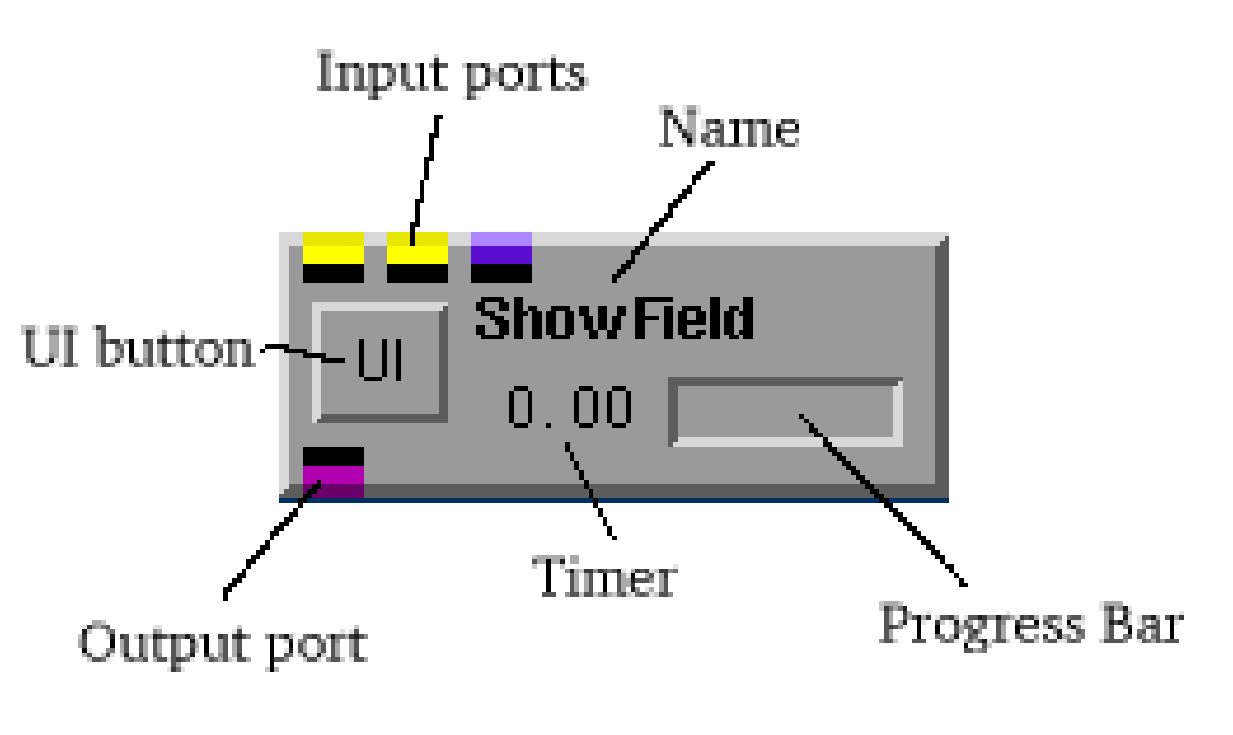
\epsfig{file=Figures/modgraphic-1.eps.gz,width=4in,
        bbllx=0, bblly=0, bburx=325, bbury=157}}}
%end{latexonly}
\begin{htmlonly}
  \newcommand{\modgraphic}{%
  \htmladdimg[align=top,width="256",alt="SCIRun Module Graphic"]
  {../Figures/modgraphic-1.gif}}
\end{htmlonly}

All modules are represented similarly by a graphic within the NetEdit frame
(see Figure~\ref{fig:modgraphic}). This graphical ``front end'' is the same
for all modules and consists of the following elements:

\begin{figure}[htb]
  \begin{makeimage}
  \end{makeimage}
  \modgraphic
  \caption{\label{fig:modgraphic} Module Graphic (\module{Show
      Field} Module)}
\end{figure}

\begin{description}
  \descitem{Module Name} The module's name.
  
  \descitem{Input Ports} Zero or more input ports located on the top
  of the module.  Each port corresponds to a data type and each data
  type has a unique color.  Table~\ref{tab:portcolors} maps port
  colors to data types.  Input ports connect to other modules' output
  ports.  Connections can only be made between ports of the same type.

  \begin{table}[htbp]
    \begin{center}
      \begin{tabular}{|l|l|}
        \hline
        \textbf{Data Type} & \textbf{Port Color} \\
        \hline
        Field & Yellow \\
        Field Set & Green \\
        Matrices & Blue \\
        Geometric Objects & Pink \\
        Color Maps & Purple \\
        Camera Path & Brown \\
        \hline
      \end{tabular}
      \caption{Data Types and their Port Colors}
      \label{tab:portcolors}
    \end{center}
  \end{table}
  
  \descitem{Output ports} Zero or more output ports located on the
  bottom of the module.  Output ports connect to other modules' input
  ports.  Every module has  at least 1 input or 1 output
  port.
  
  \descitem{UI button} Pressing the \button{UI} button displays the
  module's control dialog. Some modules have no dialog. Some have
  simple dialogs and some have complex dialogs that allow
  elaborate control over the module.  Figure~\ref{fig:moddialog} shows
  the control dialog for \module{Show Field} module.
  
  \descitem{Progress bar} Shows the module's progress.  As the module
  works toward completion of its task, the progress bar is filled
  with red, then yellow, then green.  When the Progress bar
  is green, the module is done.
  
  \descitem{Timer} Displays the amount of CPU time the module has
  consumed.  Located to the left of the progress bar.
  
  \descitem{Message Indicator} Shows the presence of messages in a
  module's log.  Colors represent message types.  Blue is for
  ``remarks'' (informational messages) and yellow is for ``warnings''
  (your attention is needed).  Click the indicator to display the
  module's log.

\descitem{Pop-up Menu} Pressing mouse button 3 while the mouse
  pointer is over a module gives access to the module's pop-up menu.  The
  pop-up menu gives access to the following items:
  \begin{description}
    \menuitemdesc{::Package\_Category\_Name\_Instance} This item is a
    label (not a selectable item).  It provides the module's name and
    the category and package to which the module belongs.  The
    ``Instance'' part is a unique number that distinguishes multiple
    instances of the same module.

    \menuitemdesc{Execute} Tells the module to
    execute (or re-execute).  The state of its input and
    output ports will cause other modules in the network to
    ``fire'' (execute) also..

    \menuitemdesc{Help} Displays the module's help window.
    
    \menuitemdesc{Notes} Displays the module's note pad.
    The user can use the note pad to document the purpose of the module in
    the current network.

    \menuitemdesc{Destroy} Destroys the module.
    
    \menuitemdesc{Show Log} Displays the module's message log.  Most
    modules will write messages to their log during the course of
    their execution.
    
    \menuitemdesc{Show Status} This item is a toggle button which
    turns off/on the display of the progress indicator.  Turning off
    the progress indicator speeds up the execution of complex
    networks.
  \end{description}
\end{description}


\subsection{Creating a Connection}
\label{sec:connectmods}

Mouse button 2 (the middle mouse button) is used to connect the output
(input) port of one module to the input (output) port of another
module.

To make a connection, position the mouse pointer over a module's input
(output) port.  Then press button 2 and drag the the mouse pointer towards
another module's output (input) port.

When button 2 is pressed, the program shows all valid connections as
black lines.  It also draws one red colored connection, which is the
connection made if  the drag is stopped by releasing 
button 2.

Make the connection by releasing button 2 when the pointer is over
the desired destination port or when the red colored connection is the
desired connection.  The connection will be drawn using the color
corresponding to the connection's data type.

Users may connect a module's output port to the input ports of 1 or more
modules by repeating the procedure just described.

\subsection{Setting Module Properties}
\label{sec:setmodprops}

%begin{latexonly}
  \newcommand{\moddialog}%
  {\centerline{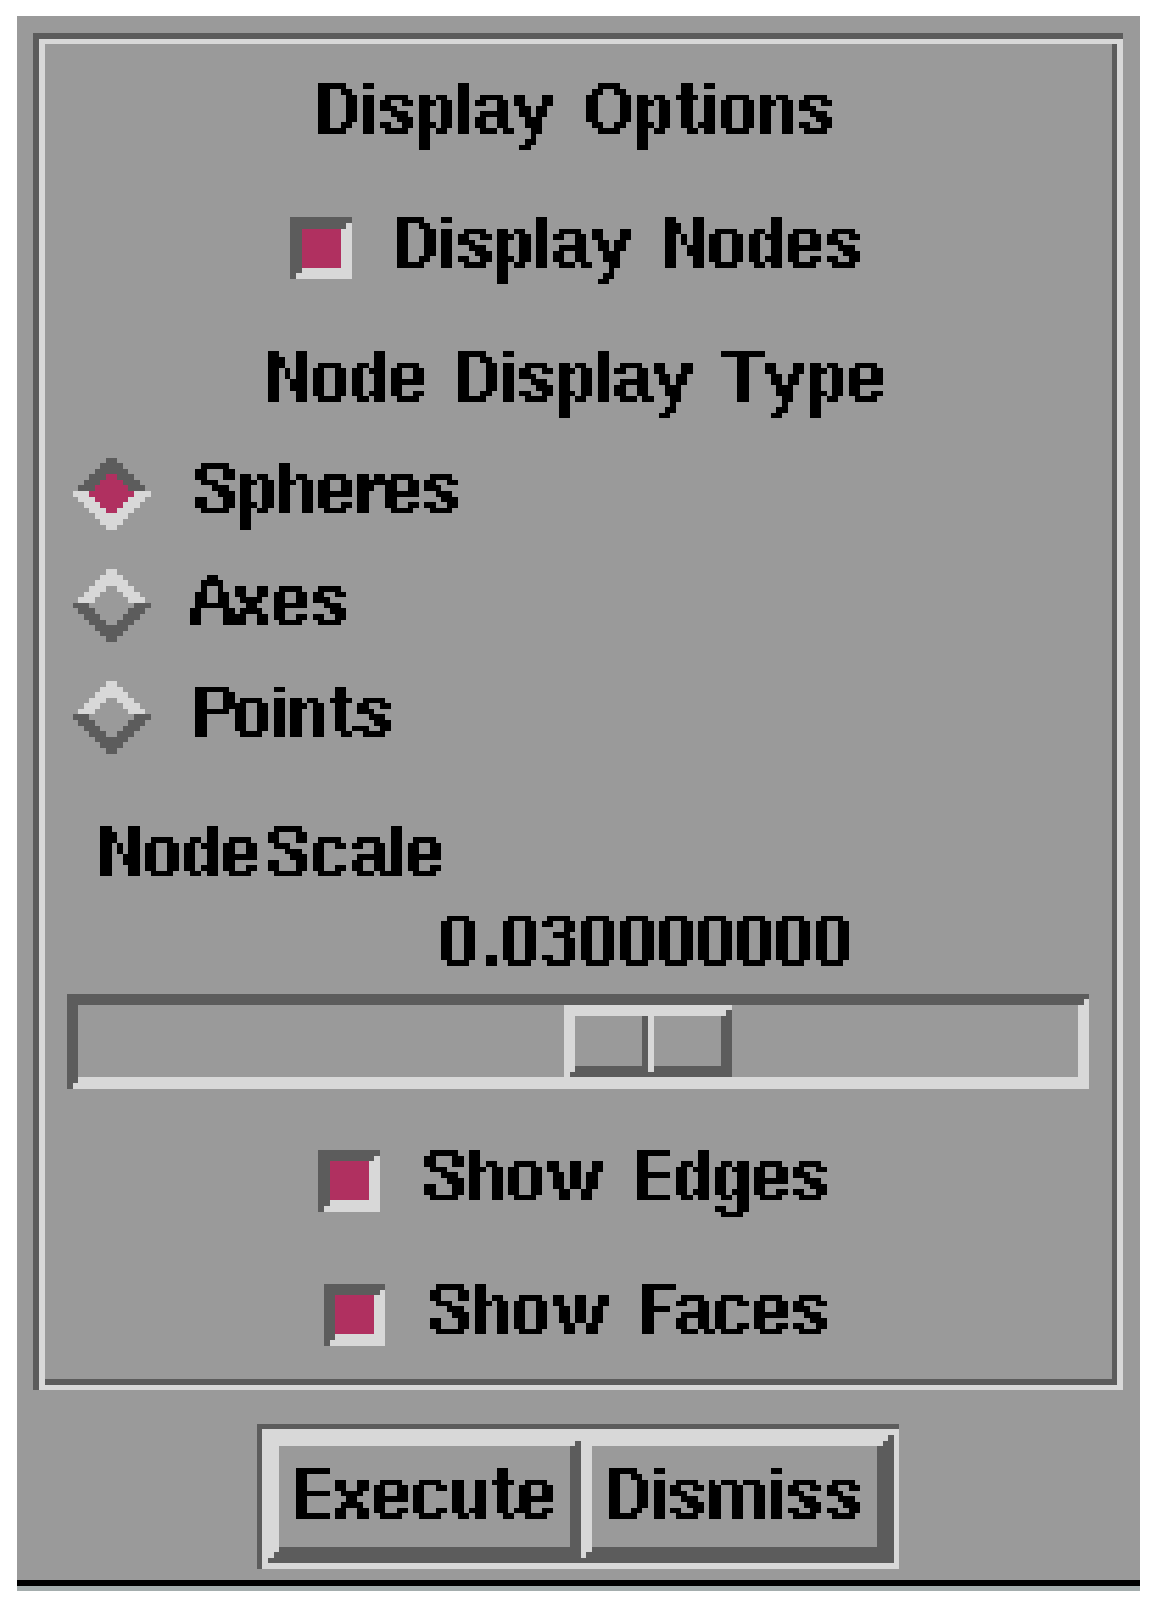
\epsfig{file=Figures/moddialog.eps.gz,
        bbllx=0, bblly=0, bburx=272, bbury=406}}}
%end{latexonly}
\begin{htmlonly}
  \newcommand{\moddialog}{%
  \htmladdimg[align=top,alt="SCIRun Module Dialog"]
  {../Figures/moddialog.gif}}
\end{htmlonly}

To change a module's properties click its \button{UI} button.  This 
displays the module's control dialog.  Use this dialog to change the
module's properties.  Each module's reference documentation explains the
use of its control dialog.  Figure~\ref{fig:moddialog} shows the control
dialog for the \module{Show Field} module.

\begin{figure}[htb]
  \begin{makeimage}
  \end{makeimage}
  \moddialog
  \caption{\label{fig:moddialog} Module \module{Show Field}'s Control Dialog
    (User Interface).}
\end{figure}

\subsection{Executing a Network}
\label{sec:executenet}

``Network Execution'' means that 1 or more modules must be executed in a
coordinated fashion. The coordinated execution of modules is managed by
\sr{}'s \dfn{scheduler}.

Note that some modules need to be compiled before they are
executed (see \secref{Dynamic Compilation}{sec:dyncomp}).  Compilation
will delay execution of the network.  This delay occurs only one time
(per module).  After a module is compiled, it does not need to be
compiled again.  Modules change color during compilation.


\subsubsection{The Basics}

The scheduler is invoked when an event occurs that \dfn{triggers} a
module's execution.  The scheduler creates a list of all modules that
must be executed in coordination with the triggered module. Modules
\dfn{upstream} (directly or indirectly) from the triggered module are 
put on the execution list if they have not previously executed.
All modules \dfn{downstream} from the triggered module are put
on the list.  Once the scheduler determines which modules must be
executed, it executes them (in parallel where possible).

Network execution is mostly transparent.  That is, the events that trigger
module execution will usually be generated automatically. Sometimes, however, the user must manually
generate a triggering event by choosing the \menuitem{Execute} item from a
module's pop-up menu.

\subsubsection{Details}

Each module executes in its own thread and blocks (waits) until its upstream
modules can supply it with data.  After a module completes its computation,
it sends its results to its downstream modules.  This completes a module's
execution cycle.  The module's next chance to receive data from its input ports
and send data to its output ports will not arise until some event
causes it to be put on the scheduler's execution list again.  

This behavior prevents modules from computing in an iterative fashion,
sending intermediate results to their downstream modules.  This is because
downstream modules cannot receive these results until they are in their
execution cycle.   Downstream modules would need to be executed each time the
upstream module posts an intermediate result.


\subsubsection{Intermediate Results}

Some modules are designed to be used in an iterative fashion.  They send
data to their output ports in a special way.  They use a method called
\icode{send\_intermediate} to send the results of each iteration.  When
this method is used, the scheduler (re)executes downstream modules each time
the upstream module posts its next result.  Downstream modules are
able to receive the results of each iteration as soon as the
upstream module sends them.

Modules \module{SolveMatrix} and \module{MatrixSelectVector} (from the
\package{\sr} package and \category{Math} category) are examples of modules
that compute iteratively using the \icode{send\_intermediate} method.

\subsubsection{Feedback Loops}

Some modules are designed to be used exclusively in feedback loops. Their output ports may be connected
directly or indirectly to their input ports.  These modules also use the
\icode{send\_intermediate} method.

Examples of feedback modules are \module{DipoleSearch} and
\module{ConductivitySearch} from the \category{Inverse} category of the
\package{BioPSE} package and \module{BuildElemLeadField} from the
\category{LeadField} category of the \package{BioPSE} package.

\subsection{Deleting a Connection}
\label{sec:deleteconnections}

Delete a connection by pressing button 3 while the pointer is
over a connection.

\subsection{Selecting Modules}
\label{sec:selectmods}

A few operations (see \secref{Moving Module(s)}{sec:movemod} and
\secref{Destroying Module(s)}{sec:destroymod}) act on a group of
modules.  A group of modules can be created in two ways

\begin{enumerate}
\item Press mouse button 2 while the pointer is in the NetEdit frame, but not over
a module or a connection.  Then drag the mouse.  This will draw a box
outline.  Modules intersecting the box will be part of the group.  Release
button 2 to complete the selection.
\item Select the first module by clicking mouse button 2 while the pointer is
over a module.  Then add modules to the group by pressing (and holding
down) the \keyboard{control} key while clicking on modules with button 2.
\end{enumerate}

Selected modules will be drawn in a darker shade of grey.

Users can mix selection methods and  add modules to the group by
pressing the control key while making selections using the above methods.
If  the control key is not pressed, then the previous group will be
forgotten and a new one will be created.

\subsection{Moving Module(s)}
\label{sec:movemod}

Modules can be moved in the NetEdit frame.  To move a module,
press button 1 while the pointer is over a module and drag the module to
its new location.

Multiple modules can be moved at one time.  To do this,
\hyperref{select}{select (see Section~}{)}{sec:selectmods} 1 or more
modules. Then press button 1 while the pointer is over any one of the
modules in the selected group and drag the modules to their new location.


\subsection{Destroying Module(s)}
\label{sec:destroymod}

Delete a module by selecting the \menuitem{Destroy} menu item from the
module's pop-up menu.

Multiple modules can be deleted at one time.  To do this,
\hyperref{select}{select (see Section~}{)}{sec:selectmods} 1 or more
modules. Then choose  \menuitem{Destroy Selected} from the module's pop-up menu.
 


\subsection{Documenting a Module's Use}
\label{sec:docmodule}

It is useful to document the purpose of a module within a network.
Each module maintains a note pad for this purpose.  Edit the
module's note pad by selecting \menuitem{Notes} from the module's
pop-up menu.  This displays the module's note pad editor.  The 
editor allows the user to write notes on the use of the
module within the context of its network.

\subsection{Viewing a Module's Log}
\label{sec:viewmodslog}

Each module supports a message log.  The module writes error messages or
other types of messages to its log.  To view this log, select the
\menuitem{Show Log} item from the module's pop-up menu.

\subsection{Documenting a Network}
\label{sec:docnetwork}

It is useful to document the function of a network.  A network's note
pad is used for this purpose.  To edit the network's note pad,
select the \menuitem{Add Info} item from the main window's \menu{File}
menu.  This will display the network's note pad editor.  The editor
allows the user to write notes on the purpose and use of the network.


\subsection{Saving a Network}
\label{sec:savenet}

\sr{} can save networks to files.  Network files have an extension of
\filename{.net} (in the past they have also had .sr and .uin
extensions).  

To save a network, select the \menuitem{Save} item from the main window's
\menu{File} menu.  A file browser dialog will prompt for the
name and location of the network file.

If  changes are made to an existing network,  \menuitem{Save} will
save changes made to an existing net file.

An existing network can be saved under a new name using the
\menuitem{Save As...} menu item.  A file browser dialog will prompt
for the new name of the network file.  Subsequent uses of
\menuitem{Save} will save changes to the newly created file.

Network files are  \dfna{Tool Command Language}{TCL} scripts.
These files can be edited, however the reasons for doing so are beyond
the scope of this guide.

\subsection{Loading a Network}
\label{sec:opennet}

To load a network file, select the \menuitem{Load} item from the main
window's \menu{File} menu.   A file browser dialog will prompt for the
name and location of the network file.

Note that loading a network file adds the network to an existing network in
the NetEdit frame, possibly overlapping the networks.

\subsection{Inserting a Network}
\label{sec:insertnetwork}

To avoid merging networks, select the
\menuitem{Insert} item from the main window's \menu{File} menu. This
option allows the user to place one \sr{} network next to another,
avoiding overlap.  A file browser dialog prompts the user for the name and
location of the network file.

The new network is inserted into the upper left corner of the
NetEdit frame.  If a network of modules already exists in the NetEdit
frame, the \menuitem{Insert} command places a new network to the
immediate right of that existing network.

\subsection{Clearing a Network}
\label{sec:clearnetwork}

Select the \menuitem{Clear} item from the main window's \menu{File}
menu in order to remove all modules and connections from the entire
NetEdit frame.  A text box appears, confirming whether the user wishes
to proceed with or cancel the clearing operation.

\subsection{Navigating a Network}
\label{sec:navnetwork}

A complex network may not be entirely visible in the NetEdit frame.
The NetEdit frame's scroll bars can be used to bring other parts of a network into
view.  Or use the network view tool to view complex networks.

The Global View Frame shows the entire ``network world.''  The small
rectangular region (outlined in black) within the Global View Frame is the
network view tool and is a window on the network world. The
position of the view tool determines the part of the network 
visible in the NetEdit frame.  To view other parts of the network, press
button 1 while the pointer is anywhere in the Global View Frame -- this 
moves the tool to the location of the pointer --  then drag the tool to the
new location.


\subsection{The \sr{} Shell}
\label{sec:termapp}

After starting, \sr{} runs a shell-like application in the terminal
window. This shell displays the prompt
\screen{scirun\ra} in the terminal window.  This program is a
\dfna{Tool Command Language}{TCL} shell program that has been extended with
\sr{} specific commands.

It is possible to type \tcl{} \sr{} commands at the prompt.  For
instance, to load a network type \keyboard{source
  \ptext{network file name}}.  This has the same effect as the \menu{File}
menu's \menuitem{Load} command.

%\incomplete{}


%%% Local Variables: 
%%% mode: latex
%%% TeX-master: t
%%% End: 

% -*-latex-*-
%
%  The contents of this file are subject to the University of Utah Public
%  License (the "License"); you may not use this file except in compliance
%  with the License.
%
%  Software distributed under the License is distributed on an "AS IS"
%  basis, WITHOUT WARRANTY OF ANY KIND, either express or implied. See the
%  License for the specific language governing rights and limitations under
%  the License.
%
%  The Original Source Code is SCIRun, released March 12, 2001.
%
%  The Original Source Code was developed by the University of Utah.
%  Portions created by UNIVERSITY are Copyright (C) 2001, 1994
%  University of Utah. All Rights Reserved.
%

%%%%%%%%%%  Figures used in this file %%%%%%%%%%%%%%%%%%%%%%%%%%%%%%%%
%% The basic viewer window
%begin{latexonly}
  \newcommand{\viewerwindow}%
  {\centerline{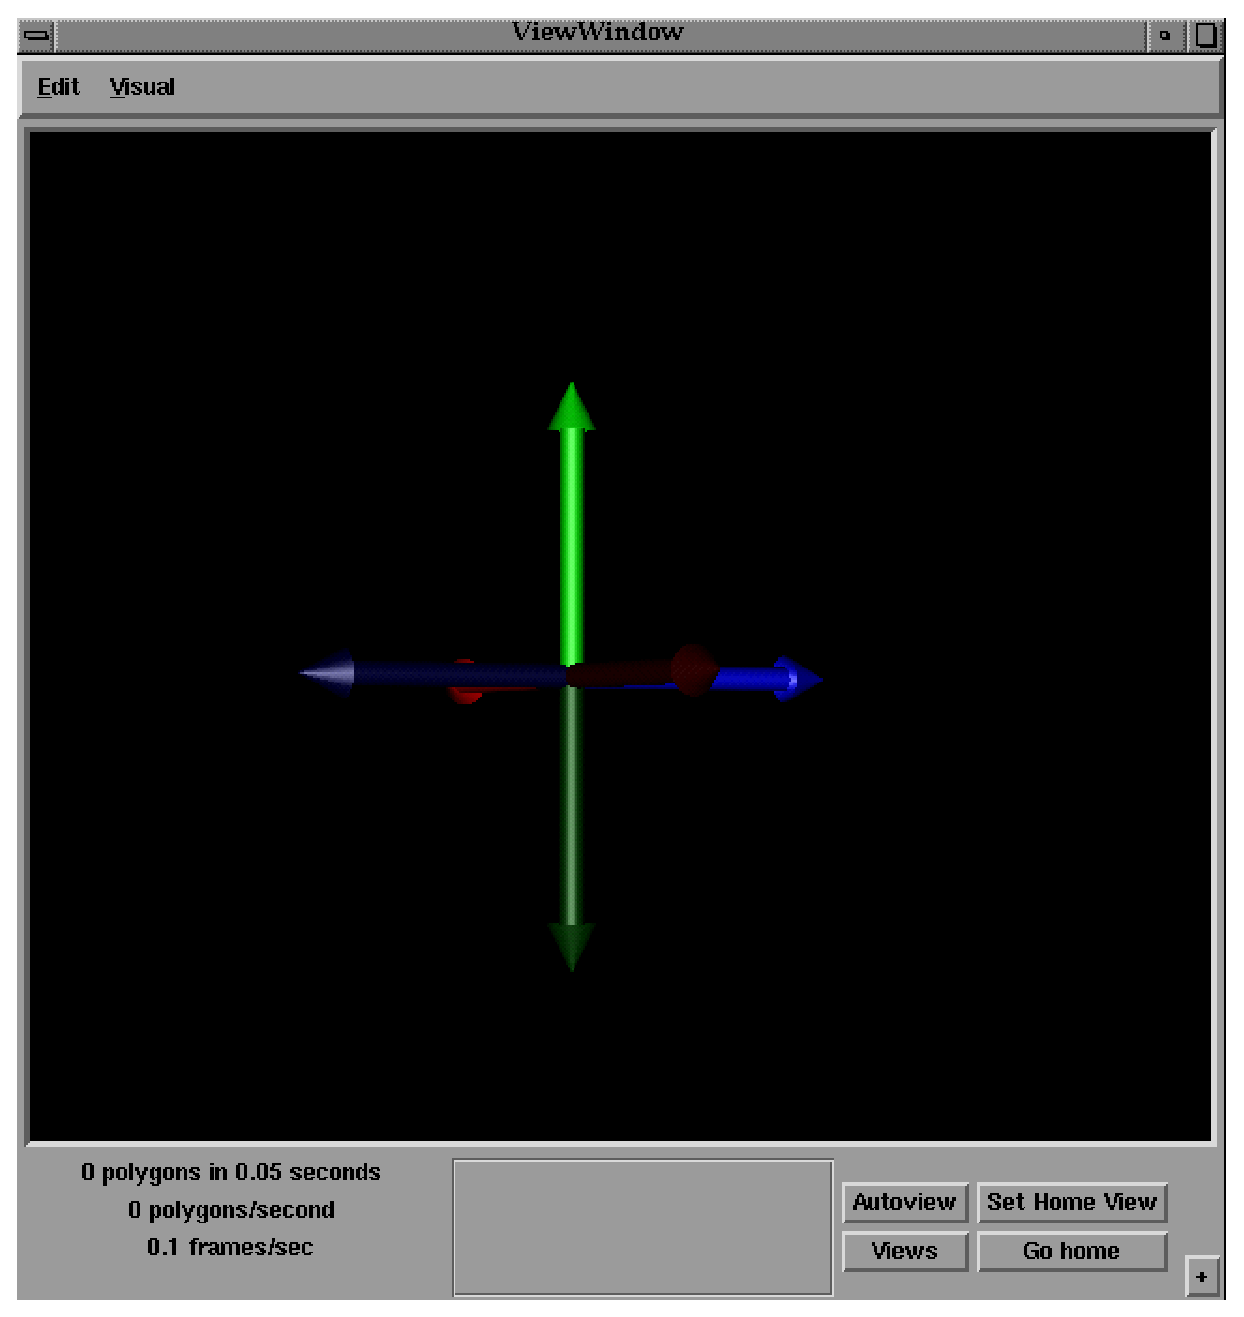
\epsfig{file=Figures/viewwindow.eps.gz,height=4in,
  bbllx=16, bblly=88, bburx=597, bbury=704}}}
%end{latexonly}
\begin{htmlonly}
  \newcommand{\viewerwindow}{%
  \htmladdimg[align=top,width=645,alt="module"]
  {../Figures/viewwindow.jpg}}
\end{htmlonly}

%% View of the extended viewer window
%begin{latexonly}
  \newcommand{\extendedwindow}%
  {\centerline{\epsfig{file=Figures/viewwindow-ext.eps.gz,height=4in,
  bbllx=16, bblly=310, bburx=600, bbury=703}}}
%end{latexonly}
\begin{htmlonly}
  \newcommand{\extendedwindow}{%
  \htmladdimg[align=top,width=649,alt="extended view window"]
  {../Figures/viewwindow-ext.jpg}}
\end{htmlonly}

%% Gauge widget image
%begin{latexonly}
  \newcommand{\gaugewidget}%
  {\centerline{\epsfig{file=Figures/widget-gauge.eps.gz,height=2in,
  bbllx=0, bblly=0, bburx=457, bbury=340}}}
%end{latexonly}
\begin{htmlonly}
  \newcommand{\gaugewidget}{%
  \htmladdimg[align=top,width=458,alt="gaugewidget"]
  {../Figures/widget-gauge.gif}}
\end{htmlonly}

%% Frame widget image
%begin{latexonly}
  \newcommand{\framewidget}%
  {\centerline{\epsfig{file=Figures/widget-frame.eps.gz,height=2in,
  bbllx=0, bblly=0, bburx=328, bbury=268}}}
%end{latexonly}
\begin{htmlonly}
  \newcommand{\framewidget}{%
  \htmladdimg[align=top,width=329,alt="framewidget"]
  {../Figures/widget-frame.gif}}
\end{htmlonly}

%% Box widget image
%begin{latexonly}
  \newcommand{\boxwidget}%
  {\centerline{\epsfig{file=Figures/widget-box.eps.gz,height=2in,
  bbllx=0, bblly=0, bburx=458, bbury=342}}}
%end{latexonly}
\begin{htmlonly}
  \newcommand{\boxwidget}{%
  \htmladdimg[align=top,width=459,alt="boxwidget"]
  {../Figures/widget-box.gif}}
\end{htmlonly}

%% Ring widget image
%begin{latexonly}
  \newcommand{\ringwidget}%
  {\centerline{\epsfig{file=Figures/widget-ring.eps.gz,height=2in,
  bbllx=0, bblly=0, bburx=507, bbury=467}}}
%end{latexonly}
\begin{htmlonly}
  \newcommand{\ringwidget}{%
  \htmladdimg[align=top,width=508,alt="ringwidget"]
  {../Figures/widget-ring.gif}}
\end{htmlonly}

%%%%%%%%%%%%%%%%%%%%%%%%%%%%%%%%%%%%%%%%%%%%%%%%%%%%%%%%%%%%%%%%%%%%%%
\newcommand{\graphics}{\emph{Graphics}}

\section{Visualization with the \viewer{}}
\label{sec:viewer}
\index{Viewer@\viewer{}}

This section describes perhaps the most frequently used module of \SR{},
the \viewer{}, which has the task of displaying interactive graphical
output to the computer screen.  You will use the \viewer{} any time you
wish to see a geometry, or spatial data.  More important for the
computational steering (described in \secref{Computational
Steering}{sec:con-steering}), is that the \viewer{} provides access to
many simulation parameters and controls and thus indirectly initiates new
iterations of the simulation steps.

We begin with an overview of the \viewer{} window and its controls, then
describe in detail all the options and variations.

\subsection{Anatomy of the \viewer{} window}
\label{sec:viewer-anatomy} 
\index{Viewer@\viewer{}!anatomy}

The \viewer{} window contains two main areas, the upper portion, called the
\graphics{} window, which displays the graphics, and the lower portion,
where most of the control buttons are.  Figure~\ref{fig:viewwindow}
contains an example of a \viewer{} window. In the \graphics{}
window, control is mostly by means of the mouse, mouse buttons, and various
modifier keys (shift/control/alt).  In the lower window are a lot of
buttons and sliders, the function of which will become clear when you read
this manual.

\begin{figure}[htb]
  \begin{makeimage}
  \end{makeimage}
  \viewerwindow
%    \framebox{\parbox[3in]{\columnwidth}{The\dotfill Figure\\
%    \vspace{2in}\\
%    With some \dotfill dummy text}}
  \caption{\label{fig:viewwindow} The default \viewer{} window in \SR{}}
\end{figure}


First, try out the controls for the \graphics{} window by moving the mouse
to the center of the viewer window and clicking and holding the left button
and then dragging the mouse.  The objects should translate along with the
mouse.  Do the same operation with the middle mouse button and the objects
will rotate around a point in the center of the display.  The right mouse
button controls the scale of the display, zooming in when the mouse moves
downward or to the right.  See \secref{Mouse Control in the
Viewer}{sec:view-mouse} for all the gory details on mouse control.

The controls visible along the bottom of the \viewer{} window set some basic
configurations as follows:
%
\begin{description}
  \item [\fbox{Autoview:} ] restores the display back to a default
        condition, very useful when some combination of settings results in
        the objects disappearing from the view window.
  \item [\fbox{Set Home View:} ] captures the setting of the current view
        so you 
        can return to it later by clicking the ``Go home'' button.
  \item [\fbox{Go home:} ] restore the current home view.
  \item [\fbox{Views:} ] lists a number of standard viewing angles and
        orientations.  The view directions align with the Cartesian axes
        of the objects and the ``Up vector'' choice sets the orientation of
        the objects when viewed along the selected axis.
\end{description}

In the left corner of the control panel of the \viewer{} window are
performance indicators that document the current rendering speed for the
display.  The better the graphics performance of the workstation you
have, the higher the drawing rate.

In the lower right corner of the \viewer{} window is a small plus sign
(``+'').  Clicking on this reveals the extended control panel with controls
that we will describe in detail in \secref{Extended control window}
{sec:view-control}.



\subsubsection{Menus}
\index{Viewer@\viewer{}!menus}

At the top of the \viewer{} window are two pull-down menus.
\begin{description}
  \item [\fbox{Edit:} ] provides access to controls for the background
        color for the window, as well as the clipping planes (requires the
        ``Use Clip'' control to be selected in the extended controls
        described in \secref{Extended control window}{sec:view-control}).
  \item [\fbox{Visual:} ] allows you to select between different graphics
        hardware settings that are available on your workstation.  The list
        is ordered heuristically from most to least useful.
\end{description}

\subsection{Mouse control in the \viewer{} window}
\label{sec:view-mouse} 
\index{Viewer@\viewer{}!mouse controls}

The mouse controls within \SR{} are extensive and flexible.  The resulting
action depends on the choice of mouse button, any simultaneous control
keys, and the way the mouse moves.  The description in
Tables~\ref{tab:view-mouse} and~\ref{tab:view-unicam} below may seem overly
complicated at first, but with a little playing, it becomes intuitive
(another way of saying you will learn it if you use it enough).

\begin{table}[htb]
\begin{center}
  \begin{tabular}{|l|l|p{5in}|} \hline
    \multicolumn{3}{|c|}{\large Mouse Controls}\\ \hline \hline 
    \multicolumn{1}{|c|}{Control Key} & 
    \multicolumn{1}{|c|}{Button} & 
    \multicolumn{1}{|c|}{Action}\\ \hline
None & Left & Translate scene \\
     & Middle & \begin{raggedleft} Rotate scene about its center on an arc
    ball that surrounds it; rotation direction is a function of the
    initial mouse location so try different sites and note the
    response. \end{raggedleft}\\  
     & Right & Zoom or scale scene (downwards and to the right increases
     size, upwards or to the left decreases size) \\ \hline
Shift & Left & Select and move a widget in the display \\
      & Middle & Toggle through the modes for a widget \\
      & Right & Pop up a widget information window \\ \hline
Control & Left & Translate in the Z-direction, \ie{} zoom in and out of the
    screen (down moves closer, up further away).  Moving left and
    right increases the ``throttle'' of the Z-direction motion.  If
    the cursor is over a point on an object when clicked, this point
    becomes the center of the screen for translation.\\ 
      & Middle & Rotate the camera view about the eye point (using arcball
    motion). \\ 
      & Right & Unicam movement (see next table)\\ \hline
\end{tabular}
\caption{\label{tab:view-mouse} Mouse controls for the \viewer{}}
\end{center}
\end{table}

\bigskip

\begin{table}
\begin{center}
\begin{tabular}{|l|l|p{3in}|} \hline
    \multicolumn{3}{|c|}{\large Unicam movement (Control key and right mouse
    button} \\ \hline \hline
    \multicolumn{1}{|c|}{Initial mouse location} & 
    \multicolumn{1}{|c|}{Action} & \\ 
    \hline
    Near edge of display & Rotate objects on the arc ball & \\
    Near the objects & Following behavior: & \\
    \hline
    & \multicolumn{1}{|c|}{Initial mouse movement} & 
    \multicolumn{1}{|c|}{Action}\\ \hline
    & Horizontal & Pan objects \\ 
    & Vertical & Zoom and pan: down = zoom in, up = zoom
    out, left and right= pan left and right) \\
    & None & Set rotation point for subsequent arc ball rotation.\\
    \hline
\end{tabular}
\caption{\label{tab:view-unicam} Autocam mouse controls in the \viewer{}}
\end{center}
\end{table}



\subsection{Extended control window}
\label{sec:view-control} 
\index{Viewer@\viewer{}!extended controls}

Click on the ``+'' sign in the lower right corner of the default
\viewer{} window, and the window expands to reveal an extended panel of
control buttons, as shown in Figure~\ref{fig:extviewwindow}.  Click on the
``-'' sign that now replaces the ``+'' and this extended panel disappears
again.  Here we describe the control options available in the extended
control window.

\begin{figure}[htb]
  \begin{makeimage}
  \end{makeimage}
  \extendedwindow
%    \framebox{\parbox[3in]{\columnwidth}{The\dotfill Figure\\
%    \vspace{2in}\\
%    With some \dotfill dummy text}}
  \caption{\label{fig:extviewwindow} The lower portion of extended
    \viewer{} window in \SR{}} 
\end{figure}


\subsubsection{Object selector}

The lower portion of the extended \viewer{} window is divided into three
columns and the middle of these contains a list of all the objects in the
display.  If the list becomes long enough, a scroll bar on the left
hand side controls which are visible.  For each entry in the list, we have
the following controls, reading from left to right:

\begin{itemize}
  \item At the left end of each of the
        objects in the list is box that displays red when that object is
        selected.  The \viewer{} window only displays those objects that
        are selected.
  \item Next comes the name of the object.
  \item The \fbox{Shading} control box that comes next determines the
        shading options that will be used for rendering the object.
        Options include: Lighting, BBox, Fog, Use Clip, Back Cull, and
        Display List (for descriptions, see
        \secref{Rendering controls}{sec:view-rendering}).
  \item As the right end of each entry is the lighting control, initially
        marked \fbox{Default}.  In the Default setting, the common
        rendering controls described in \secref{Rendering
        controls}{sec:view-rendering} below apply.  Clicking this box
        reveals a set of options that will apply only to this object that
        include Wire, Flat and Gouraud.
\end{itemize}


\subsubsection{Rendering controls}
\label{sec:view-rendering} 
\index{Viewer@\viewer{}!rendering}

The left column of the extended \viewer{} window contains controls that
apply to all of the selected objects with ``Default'' lighting selected.
Those without the Default setting will use their own, object specific
settings, as described in the previous section.  The lighting and shading
options available are:
%
\begin{description}
  \item [Lighting: ] toggles whether or not the \viewer{} applies lighting
        to the display.  Objects without lighting have a constant
        color.
  \item [Fog: ] draws objects with variable intensity based on their
        distance from the user, also known as ``depth cueing''.  Close
        objects appear brighter while more remote objects fade gradually
        into the background as a function of distance from the front.
  \item [BBox: ] toggles whether the \viewer{} draws the selected objects
        in full detail or as a simple bounding box.
  \item [Use Clip: ] applies up to six clipping planes to the display.
        To control the clipping plane locations, use the
        ``Edit -> Clipping Planes'' menu at the top.
  \item [Back Cull: ] displays only the forward facing facets of any surface
        objects in the display.
  \item [Display List: ] cache the list of objects to be displayed; this
        option accelerates rendering when the content of the display does
        not change. 
  \item [Shading: ] selects the type of shading for objects from the
        following options:
        \begin{description}
          \item [Wire: ] show only the wire mesh of objects.
          \item [Flat: ] draw each facet with a constant color.
          \item [Gouraud: ] linearly interpolate the color across facets. 
        \end{description}
\end{description}

The right hand column of the extended \viewer{} window contains controls
for displaying the axes and creating stereoscopic rendering.  

\paragraph{Stereo viewing: } requires hardware LCD glasses synchronized
with the display so that visibility for each eye coincides with the
display of the appropriate view.  The ``Fusion Scale'' control provides a
means of setting the eye separation and thus setting the view that is most
suited to facial anatomy and distance from the screen.

\subsubsection{Making movies}
\label{sec:view-movies} 
\index{movies}

The \viewer{} window in \SR{} has simple controls for capturing sequences
of images into animations or movies.  Here we describe how this works.

In the left column of the extended \viewer{} window are controls for
selecting movie type and then initiating and stopping the acquisition of
individual frames in the movie.

\SR{} sends a frame to the movie after each ``redraw'' operation, \ie{}
each time anything moves in the display or any visualization parameter
changes.  If the MPEG package is available (See the
\htmladdnormallink{Installation Manual}{\installguideurl} for
details) then an option will be available for saving the animations as MPEG
movies.

There is also a button that forces the size of the graphical window to be
352x240 pixels in size, which is a standard format well suited to MPEG.

\subsection{Control widgets}
\label{sec:view-widgets} 

While the \hyperref{mouse controls}{mouse controls in
Section}{}{sec:view-mouse} describe many ways to interact with the contents
of the \viewer{}, SR{} also supports some powerful display widgets.
Examples of widgets capabilities include managing cutting surfaces colored
according to the local data values, displaying streamlines in vector
fields, or selecting sub-volumes within the display area for further
manipulation. 
 
We have tried to make interacting with these widgets as consistent as
possible so that, for example, controlling parameters is usually by clicking
and dragging on either a cylindrical ``collar'' or a sphere element of the
widget.  The original design of these modules was by James Purcifal
%%\cite{??}. 
Note that a single widget may have more than one purpose
depending on the context in which it exists.

In this section, we describe the widgets available within \SR{} and \PSE{}.
The same widget may, for example, select a clipping or a display plane
through a three-dimensional object but may also set the seed points for a
streamline module.  

\subsubsection{Gauge Widget}
\label{sec:view-gaugewidget} 

\begin{figure}[htb]
  \begin{makeimage}
  \end{makeimage}
  \gaugewidget
%    \framebox{\parbox[3in]{\columnwidth}{The\dotfill Figure\\
%    \vspace{2in}\\
%    With some \dotfill dummy text}}
  \caption{\label{fig:gaugewidget} The gauge widget for setting location and
    density of seed points}
\end{figure}

\paragraph{Appearance: } The Gauge Widget consists of two spheres (A)
connected by a cylinder (B) with a small slider collar (C) on the cylinder.
There are also small resize cylinders extending from the spheres (D).

\paragraph{Purpose:} The primary use of the Gauge Widget is to set the
location and density of streamlines emerging from the long cylinder.  It
may also be used as a more general purpose three-dimensional slider or as a
source for a stream surface. 

\paragraph{Controls: } Clicking and dragging either sphere causes the
entire widget to move in space, rotating about the other sphere and
following along behind the selected sphere.  Dragging either of the resize
cylinders cases the size of the widget to change and dragging any point on
the main cylinder moves the whole widget without any change in orientation.
Dragging the slider collar changes the associated value, typically the
density of seed points for a streamline source.

\subsubsection{Frame Widget}
\label{sec:view-framewidget} 

\begin{figure}[htb]
  \begin{makeimage}
  \end{makeimage}
  \framewidget
%    \framebox{\parbox[3in]{\columnwidth}{The\dotfill Figure\\
%    \vspace{2in}\\
%    With some \dotfill dummy text}}
  \caption{\label{fig:framewidget} The frame widget for selecting
    cutting/projection planes}
\end{figure}


\paragraph{Appearance: } The Frame Widget consists of four cylinders
connected in a rectangle.  In the middle of each of the cylinders there is
a sphere (B), from which a resize cylinder extends (C).

\paragraph{Purpose:} The primary uses of the Frame Widget is for image
plane definition, for defining stream volumes, and as a "tie dye" as with
the Ring Widget described in \secref{Ring Widget}{sec:view-ringwidget}.

\paragraph{Controls: } Clicking and ragging a sphere on the widget will
cause the widget to rotate about it center; dragging on a resize cylinder
will move the associated edge and this extend or contract the rectangle.
Dragging any of the cylinder will drag the entire widget through space.


\subsubsection{Box Widget}
\label{sec:view-boxwidget} 

\begin{figure}[htb]
  \begin{makeimage}
  \end{makeimage}
  \boxwidget
%    \framebox{\parbox[3in]{\columnwidth}{The\dotfill Figure\\
%    \vspace{2in}\\
%    With some \dotfill dummy text}}
  \caption{\label{fig:boxwidget} The boxwidget for selecting sub-volumes}
\end{figure}

\paragraph{Appearance: } The Box Widget consists of twelve cylinders (A)
connected in a hexahedral box (three-dimensional rectangle) with cylinders
indicating on the edges of the box (B).  In the middle of each face of the
box is a sphere with a cylinder protruding from it (C) that provide resize
control.

\paragraph{Purpose:} The primary use of the Box Widget is to select a
subvolume of the workspace for further manipulation (\eg{} volume
rendering, isosurfaces, streamlines, mesh adaption) where the faces of the
widget act as orthogonal clipping planes.

\paragraph{Controls: } Clicking and dragging on one of the spheres rotates
the widget about its center without changing the position of the center.
Clicking on and dragging any resize handle
% What do these look like??
causes the associated face to extend without changing its orientation.
Dragging a cylinder causes the entire widget to move without changing its
orientation.

\subsubsection{Ring Widget}
\label{sec:view-ringwidget} 

\begin{figure}[htb]
  \begin{makeimage}
  \end{makeimage}
  \ringwidget
%    \framebox{\parbox[3in]{\columnwidth}{The\dotfill Figure\\
%    \vspace{2in}\\
%    With some \dotfill dummy text}}
  \caption{\label{fig:ringwidget} The ring widget for selecting
    cutting/projection planes}
\end{figure}


\paragraph{Appearance: } The Ring Widget consists of a ring (A) with four
embedded spheres (B), each with a resize cylindrical attached (D).  Between
two of the spheres is a sliding collar (C).  One of the resize cylinders
has a special material property (typically a different color from the other
cylinders) to indicate that it is the ``halfway point'' for the slider (E).

\paragraph{Purpose:} The primary use of the Ring Widget is to set the
density of streamlines emerging from the ring---the ring serves as a set of
seed points from which will emerge streamlines.  The Ring Widget can also
serve as a three-dimensional angle gauge, as a source for multiple
streamlines throughout its surface, as a source for a stream surface from
the outer ring, and as a source for a stream volume.  Another use is as a
color sheet, or ``tie dye'', in which the surface is colored as a function of
the scalar value of the field at each point.

\paragraph{Controls: } Clicking and dragging the slider collar along the
ring changes the density of the seed points or some other related
parameter.  Dragging the spheres controls the orientation of the Ring
Widget, while moving the resize cylinders changes the radius of the Ring
Widget about its center.  Dragging any other point on the ring moves the
ring in space without changing its radius or orientation.


%%% Local Variables: 
%%% mode: latex
%%% TeX-master: t
%%% End: 

% package.tex
%

\section{Packages}
\label{sec:packages}

\missing{}

\subsection{The SCIRun Package}
\label{sec:srpackage}

\begin{description}
\item[\package{DataIO}] \missing{}
\item[\package{Fields}] \missing{}
\item[\package{Math}] \missing{}
\item[\package{Render}] \missing{}
\item[\package{Visualization}] \missing{}
\end{description}

\subsection{The BioPSE Package}
\label{sec:biopsepackage}

\begin{description}
\item[\package{Forward}] \missing{}
\item[\package{Inverse}] \missing{}
\item[\package{LeadField}] \missing{}
\item[\package{Visualization}] \missing{}
\end{description}

%%% Local Variables: 
%%% mode: latex
%%% TeX-master: "usersguide"
%%% End: 

%\input{ui}
% -*-latex-*-
%
%  The contents of this file are subject to the University of Utah Public
%  License (the "License"); you may not use this file except in compliance
%  with the License.
%
%  Software distributed under the License is distributed on an "AS IS"
%  basis, WITHOUT WARRANTY OF ANY KIND, either express or implied. See the
%  License for the specific language governing rights and limitations under
%  the License.
%
%  The Original Source Code is SCIRun, released March 12, 2001.
%
%  The Original Source Code was developed by the University of Utah.
%  Portions created by UNIVERSITY are Copyright (C) 2001, 1994
%  University of Utah. All Rights Reserved.
%

\section{Importing data into \sr{}}
\label{sec:import} 
\index{importing}

Here we describe some of the channels through which you can import data
into \sr{}.  The basic paradigm a this point requires converting existing
files into standard \sr{} files.  We will extend this very soon to support
readers within \sr{} that will accept other formats.


\subsection{CVRTI converters}

The Cardiovascular Research and Training Institute (CVRTI) has developed a
number of scalar and vector data and geometry file formats which required
converters for \sr{}.  The result is a set of stand-alone programs that read
in one more more existing CVRTI files and generate a particular form of
\sr{} file, the details of which depend on the particular combination of
nodes, connectivities, and associated attributes.

The programs and their parameters as as follows (go to the end of the list
to see the definitions of the different parameter and file types):
%
\begin{description}
  \item [CVRTItoTriSurfGrad: ] converts nodes, triangle connectivities, and
        vector (grad) files into a field with associated vector attribute:\\
        \begin{verbatim}
        CVRTItoTriSurfGrad pts fac grad [channels] fieldout
        \end{verbatim}
  \item [CVRTItoTriSurfPot: ] converts nodes, triangle connectivities, and
        scalar (pot) data files into a field with associated scalar
        attributes. 
        \begin{verbatim}
        CVRTItoTriSurfPot pts fac pot [channels] fieldout
        \end{verbatim}
  \item [CVRTItoTetVolGrad: ] converts nodes, tetrahedral connectivities, and
        vector (grad) files into a field with associated vector
        attributes:\\
        \begin{verbatim}
        CVRTItoTetVolGrad pts tetras grad [channels] fieldout
        \end{verbatim}
  \item [CVRTItoTetVolPot: ] converts nodes, tetrahedral connectivities, and
        scalar (pot) files into a field with associated scalar attributes:\\
        \begin{verbatim}
        CVRTItoTetVolPot pts tetras pot [channels] fieldout
        \end{verbatim}
\end{description}

\paragraph{Definitions:}

\begin{center}
\begin{tabular}{|c|p{4in}|} \hline
\multicolumn{1}{|c|}{Argument} &
\multicolumn{1}{|c|}{Purpose} \\ \hline
\multicolumn{2}{|l|}{Geometry} \\ \hline
pts & CVRTI points file; ASCII file with one x,y,z triplet per line.*\\
fac & CVRTI triangle connectivity (facet) file; ASCII file with one
    triangle defined per line.  Each value points to a node number in the
    associated .pts file, with 1 (not 0) as the first node number.*  \\
tetras & CVRTI tetrahedra file; ASCII file with the nodes from one
    tetrahedron on each line, pointing to the nodes in the associated .pts
    file.  Pointers begin with 1 (not 0).*\\ \hline
\multicolumn{2}{|l|}{Data} \\ \hline
grad & CVRTI vector file; ASCII file with two x,y,z triplets per line;
    first triplet is origin of the vector and second is the endpoint.*\\
pot & CVRTI scalar (potentials) data file; ASCII file,  each line contains
    one scalar value.  Without .channels file, all programs assume a
    one-to-one mapping of scalar value to the  nodes in the associated .pts
    file.*\\ \hline
\multicolumn{2}{|l|}{Channel Mapping} \\ \hline
channels & CVRTI data channel mapping file; ASCII file that begins with the
    line ``N channels'', where N is the number of channels in the file.
    Subsequent lines contain two values, the first refers to a node number in
    the geometry and the second points to the associated channel of any scalar
    or vector data files.  Thus a .channels file must have an entry for each
    node of the associated .pts file but the associated .pot file can have more
    (or even fewer) entries.\\ \hline
\multicolumn{2}{|l|}{Field File} \\ \hline
field & SCIRun fields file that contains both the geometry and associated
    scalar or vector data as attributes. \\ \hline
& *\textbf{Note}: to find the length of all CVRTI ASCII geometry,
scalar, and vector files, count the number of lines in the file. \\
\hline
\end{tabular}
\end{center}

\paragraph{Location of converter programs:}
All converter programs are normally available in the subdirectory of the
\sr{} distribution called \directory{src/StandAlone/convert}.  If they are
not easily available, ask the local person who installed \sr{} for
assistance.

%\input{samples}

% Now the glossary, appendiced, bibliography, and index
\newpage
%\chapter{Glossary} \label{Sec:Glossary}

\begin{itemize}

\item Data Warehouse (NewDW, OldDW, DW) - The \tt Data Warehouse
         \normalfont is an abstraction (and implementation vehicle) used in
         Uintah to provide data to simulation components (across
         distributed memory spaces as necessary).  OldDW refers to a
         DW from the previous time step.  NewDW refers to the DW for
         the current time step.  In practice, variables are usually
         pulled from the OldDW, updated, and placed in the NewDW.

\item Time step - Uintah is a time dependent code.  A time step refers
         to a unique point in simulation time.  The state of the
         simulation is updated one time step at a time.
         
\item Adaptive Mesh Refinement (AMR) - In brief, AMR allows spending
  less CPU time on ``inactive'' (less interesting) areas of the
  simulation, and spend more time computing where there are many
  particles reacting.  Resolution is low in the center where things
  are stable, but high at the edges.  This feature is in ICE, but not
  ARCHES.

\item CCA - Common Component Architecture.

\item CFD - Computational Fluid Dynamics modeling.

\item DistCC - Parallel, distributed compiler.

\item Doxygen - Doxygen (code documentation) web interface.

\item GhostCells (and Extra Cells)

\item Grid - The problem's physical domain.  The number of cells in the
  grid determine the resolution of the simulation.

\item Handle - Smart pointers.  Handles track the number of references
  to a given object, and when the number reaches zero, de-allocates
  the memory.

\item Level - Not a 'level' in 3d-space, but a level of recursion into an
  AMR grid.  ARCHES doesn't support AMR or nonuniform cells, and
  therefore doesn't need recursion, so it works on a single level '1'.

\item Material Point Method (MPM) - The main component for simulating
  structures (physcial objects) in the UCF.

\item Message Passing Interface (MPI) - Communication library used by many
  distributed software packages to communicate data between multiple
  processors.  Besides send'ing and recv'ing data, data
  reduction (UCF Reduction Variables) is supported. 
  \begin{itemize}
    \item OpenMPI
  \end{itemize}

\item Patch - A physical region of the grid assigned one to each
  processor.  The processor working on a patch will compute properties
  for each of the cells contained in the patch.  Think of this as a big
  cube that contains hundreds of little cubes.

\item Regression Tester (RT) - Runs nightly accuracy, memory, and
  completion tests on Uintah simulations.

%\item <table border=''1'' cellpadding=''5'' width=''80%''><tr><td
%                                %bgcolor=''#eeeeff''><b>Programmers
%                                %Note:</b> Programming examples and
%                                %notes will appear like
%                                %this.</td></tr></table>

\item SCIRun - A Problem Solving Environment (PSE) originally used to
  provide core software building blocks for Uintah as well as an
  extensive visualization package for viewing Uintah data archives.

\item SUS - Standalone Uintah Simulator.  This is the main executable
  program in the Uintah project.

\item SVN - Subversion code versioning system.

\item Uintah - The general name of the C-SAFE simulation code.
  Sometimes also refered to as the UCF.  The name comes from the
  Uintah mountain range in Utah.

\item Uintah Computational Framework (UCF) - The core software
  infrastructure for Uintah.
  \begin{itemize}
    \item Variables (CC, NC, FC) - Cell centered, Node centered, and
      Face centered (respectively) data structures used within the UCF.
  \end{itemize}

\item Uintah Data Archive (UDA) - The directory/file/data layout for
  storing Uintah simulation data.

\item Uintah Problem Specification (UPS (Section~\ref{Sec:UPS})) - An XML based file used to
  specify Uintah simulation properties.

\item Uintah Software Organization
  \begin{itemize}
    \item Visualization
    \item scinew - a wrapper for the C++ new() function that allows for memory tracking.
  \end{itemize}

\end{itemize}


% Appendicies
\newpage
% \section*{Appendicies}
% \subsection*{Appendix A. Bomb Units} \label{appendixBombUnits}
\appendix
\addappheadtotoc

\chapter{Bomb Units} \label{appendixBombUnits}

Following is a table of conversion factors from bomb units to mks units.  Bomb units are useful in small scale
simulations that occur very quickly, such as detonation and deformation. \\

\begin{tabular}{|c|c|}
\hline 
\bf{Measure} & \bf{Conversion Factor}     \\
\hline
mass	& $\mu g$               \\
length  & cm                    \\
time    & $\mu s$               \\ [1ex]
kinematic viscosity & $1\frac{\displaystyle cm^2}{\displaystyle \mu s} = 10^2 \frac{\displaystyle m^2}{\displaystyle s}$                          \\ [1ex]
velocity            & $1\frac{\displaystyle cm}{\displaystyle \mu s} = 10^4 \frac{\displaystyle m}{\displaystyle s}$                              \\ [2ex]
force               & $1\frac{\displaystyle \mu gcm}{\displaystyle \mu s^2} = 10 N$                                                               \\ [2ex]
pressure            & $\frac{\displaystyle 10 N}{\displaystyle cm^2} = 10^5 Pa$                                                                   \\ [1ex]
viscosity           & $10^5 Pa \mu s = 10^{-1} Pa s$                                                                                              \\ [1ex]
density             & $1\frac{\displaystyle \mu g}{\displaystyle cm^3} = 1\frac{\displaystyle g}{\displaystyle m^3}$                              \\ [1ex]
heat capacity       & $\frac{\displaystyle 10N cm}{\displaystyle \mu g K} = 10^8 \frac{\displaystyle J}{\displaystyle kg K}$                      \\ [2ex]
power               & $\frac{\displaystyle 10N cm}{\displaystyle \mu s} = 10^5 W$                                                                 \\ [1ex]
thermal conductivity& $\frac{\displaystyle 10^5 W}{\displaystyle cm K} = 10^7 \frac{\displaystyle W}{\displaystyle m K}$                          \\ [2ex]
surface energy      & $\frac{\displaystyle 10 N cm}{\displaystyle cm^2} = 10^3 \frac{\displaystyle J}{\displaystyle m^2}$                         \\ [2ex]
fracture toughness  & $\frac{\displaystyle 10 N}{\displaystyle cm^{\frac{3}{2}}} = 10^{-2} \frac{\displaystyle N}{\displaystyle m^{\frac{3}{2}}}$ \\ [2ex]
enthalpy            & $1\frac{\displaystyle J}{\displaystyle kg} = 10^{-8} \frac{\displaystyle cm^2}{\displaystyle \mu s^2}$                      \\ [2ex]
\hline
\end{tabular}



\newpage
%\input{appendices}

\newpage
\bibliography{biglit,crj,mm}
\bibliographystyle{unsrt}
\newpage
\printindex
\end{document}
